% ============================================================
% Market Power and the Gender Career Gap
% Field Exam Presentation
% ============================================================
\documentclass[aspectratio=169, 11pt]{beamer}

% ---------- theme & colors ----------
\usetheme{default}
\usecolortheme{default}
\setbeamertemplate{navigation symbols}{}
\setbeamertemplate{footline}[frame number]

% Colors matching academic-pptx palette
\definecolor{navy}{HTML}{1F4E79}
\definecolor{accentblue}{HTML}{2E75B6}
\definecolor{bodytext}{HTML}{2D2D2D}
\definecolor{muted}{HTML}{777777}
\definecolor{lightbg}{HTML}{EBF3FA}
\definecolor{rulecolor}{HTML}{CCCCCC}
\definecolor{faded}{HTML}{BBBBBB}
\definecolor{midblue}{RGB}{46, 117, 182}

\setbeamercolor{frametitle}{fg=navy}
\setbeamercolor{title}{fg=navy}
\setbeamercolor{normal text}{fg=bodytext}
\setbeamercolor{structure}{fg=accentblue}
\setbeamercolor{itemize item}{fg=accentblue}
\setbeamercolor{itemize subitem}{fg=muted}

\setbeamerfont{frametitle}{series=\bfseries, size=\large}
\newcommand{\bmark}[1]{\textcolor{midblue}{\textbf{#1}}}

% ---------- frametitle rule ----------
\setbeamertemplate{frametitle}{%
  \vspace{0.3cm}%
  {\usebeamerfont{frametitle}\usebeamercolor[fg]{frametitle}\insertframetitle}\\[-4pt]%
  {\color{rulecolor}\rule{\textwidth}{0.4pt}}%
  \vspace{0.05cm}%
}

% ---------- packages ----------
\usepackage{booktabs}
\usepackage{graphicx}
\usepackage{hyperref}
\usepackage{amsmath,amssymb}
\usepackage{tikz}
\usetikzlibrary{positioning, arrows.meta, decorations.pathreplacing}
\usepackage[T1]{fontenc}
\usepackage{lmodern}
\usepackage{bbm}
\usepackage{comment}

% ---------- figure path shortcut ----------
\graphicspath{{../../../1_Code/figures/}}

% ============================================================
\title{Market Power and the Gender Career Gap:\\Evidence from Matched HR Records in Chile}
\author{Sofia Valdivia}
\institute{Duke University}
\date{Field Exam --- \today}

\begin{document}

% ============================================================
% SLIDE 1: Title
% ============================================================
{
\setbeamercolor{background canvas}{bg=white}
\begin{frame}[plain]
\vfill
\begin{center}
{\Large\bfseries\textcolor{navy}{Market Power and the Gender Career Gap}}\\[6pt]
{\large\textcolor{navy}{Evidence from Matched HR Records in Chile}}\\[20pt]
{\normalsize\textcolor{navy}{Sofia Valdivia}}\\[4pt]
{\small\textcolor{navy}{Duke University}}\\[16pt]
{\small\textcolor{navy}{Field Exam --- \today}}
\end{center}
\vfill
\end{frame}
}

% ============================================================
% SECTION A: Motivation
% ============================================================

\begin{frame}
\frametitle{Wages are only one dimension of how careers unfold}

\begin{itemize}
    \item Gender gaps persist despite convergence in education and declining fertility (Goldin, 2014; Blau \& Kahn, 2017). Most research focuses on \emph{wages}, but firms also decide \textbf{who gets hired} and \textbf{who gets promoted}.

    \medskip
    \item Search frictions give firms market power over workers (Manning, 2003). Women face fewer outside options than men (Webber, 2016; Caldwell \& Danieli, 2022). \bmark{This depresses wages --- but does it also distort hiring and promotion decisions?}

    \medskip
    \item \textbf{The mechanism:} A firm deciding whether to promote weighs the output gain against the wage increase --- but also \emph{retention}. If a male worker has many outside options, the firm promotes to keep him. If a female worker has fewer options, the firm can delay at little cost.

    \medskip
    \item \textbf{This paper:} connects imperfect competition to gender gaps in career dynamics at \emph{both} the hiring and promotion margins, using matched employer-employee-applicant data from Chile.
\end{itemize}

\end{frame}

% ============================================================
% SECTION B: Setting & Data
% ============================================================

\begin{frame}
\frametitle{Chile: convergence in education and fertility, persistence in gaps}

\begin{itemize}
    \item Women surpassed men in tertiary attainment (45\% vs.\ 37\%), TFR fell to 1.03 --- yet the gender wage gap persists at 15--20\% and female labor force participation remains at 53\% (OECD avg: 65\%)

    \medskip
    \item These gaps have become a central policy concern, prompting a series of \textbf{labor market reforms} during the 2022--2026 period:
    \begin{itemize}
        \item \textbf{40-hour workweek} (Ley 21.561, phased 2024--2028) --- changes the premium on long-hours availability
        \item \textbf{Flexible work for caregivers} (Ley 21.645, Jan 2024) --- parents of children under 14 can request remote/flexible work
        \item \textbf{Childcare mandate} (Art.\ 203) --- firms with $\geq$20 female workers must fund childcare; firms bunch at 19
    \end{itemize}

    \medskip
    \item Each reform shifts a different \textbf{parameter of the firm's problem} and can be exploited for identification
\end{itemize}

\end{frame}

% --- BUK pipeline ---
\begin{frame}[label=bukslide]
\frametitle{BUK records the full employment relationship}

\textbf{BUK} is an HR and payroll platform used by 19,000+ Chilean firms across all 20 ISIC sectors. It records each stage of the employment relationship:

\vspace{0.3cm}
\begin{center}
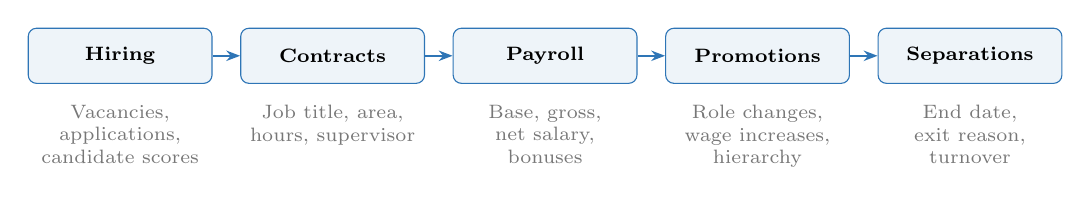
\begin{tikzpicture}[node distance=0.15cm and 0.35cm,
  box/.style={draw=accentblue, rounded corners=3pt, fill=accentblue!8,
              text width=2.1cm, align=center, minimum height=0.7cm, font=\scriptsize\bfseries},
  sub/.style={text width=2.1cm, align=center, font=\scriptsize\color{muted}},
  arr/.style={-{Stealth[length=5pt]}, thick, accentblue}]
  \node[box] (hire) {Hiring};
  \node[box, right=of hire] (contract) {Contracts};
  \node[box, right=of contract] (pay) {Payroll};
  \node[box, right=of pay] (promo) {Promotions};
  \node[box, right=of promo] (exit) {Separations};
  \draw[arr] (hire) -- (contract);
  \draw[arr] (contract) -- (pay);
  \draw[arr] (pay) -- (promo);
  \draw[arr] (promo) -- (exit);
  % sublabels
  \node[sub, below=of hire] {Vacancies,\\applications,\\candidate scores};
  \node[sub, below=of contract] {Job title, area,\\hours, supervisor};
  \node[sub, below=of pay] {Base, gross,\\net salary,\\bonuses};
  \node[sub, below=of promo] {Role changes,\\wage increases,\\hierarchy};
  \node[sub, below=of exit] {End date,\\exit reason,\\turnover};
\end{tikzpicture}
\end{center}

\vspace{0.2cm}
\begin{itemize}
    \item \textbf{Worker--month panel:} 4.7M workers, 8.3M job spells, with firm, occupation, and supervisor identifiers
    \item \textbf{Recruitment module:} 186K selection processes, 2.7M applications --- observe the hiring pipeline from application through scoring
    \item \textbf{Complemented by} the Work in Progress survey (perceptions, satisfaction, preferences) \hyperlink{survey}{\beamergotobutton{Survey details}}
\end{itemize}

\end{frame}

% --- Panel coverage and reform timeline ---
\begin{frame}
\frametitle{Panel coverage and reform timeline (2022--2026)}

\vspace{-0.1cm}
\begin{center}
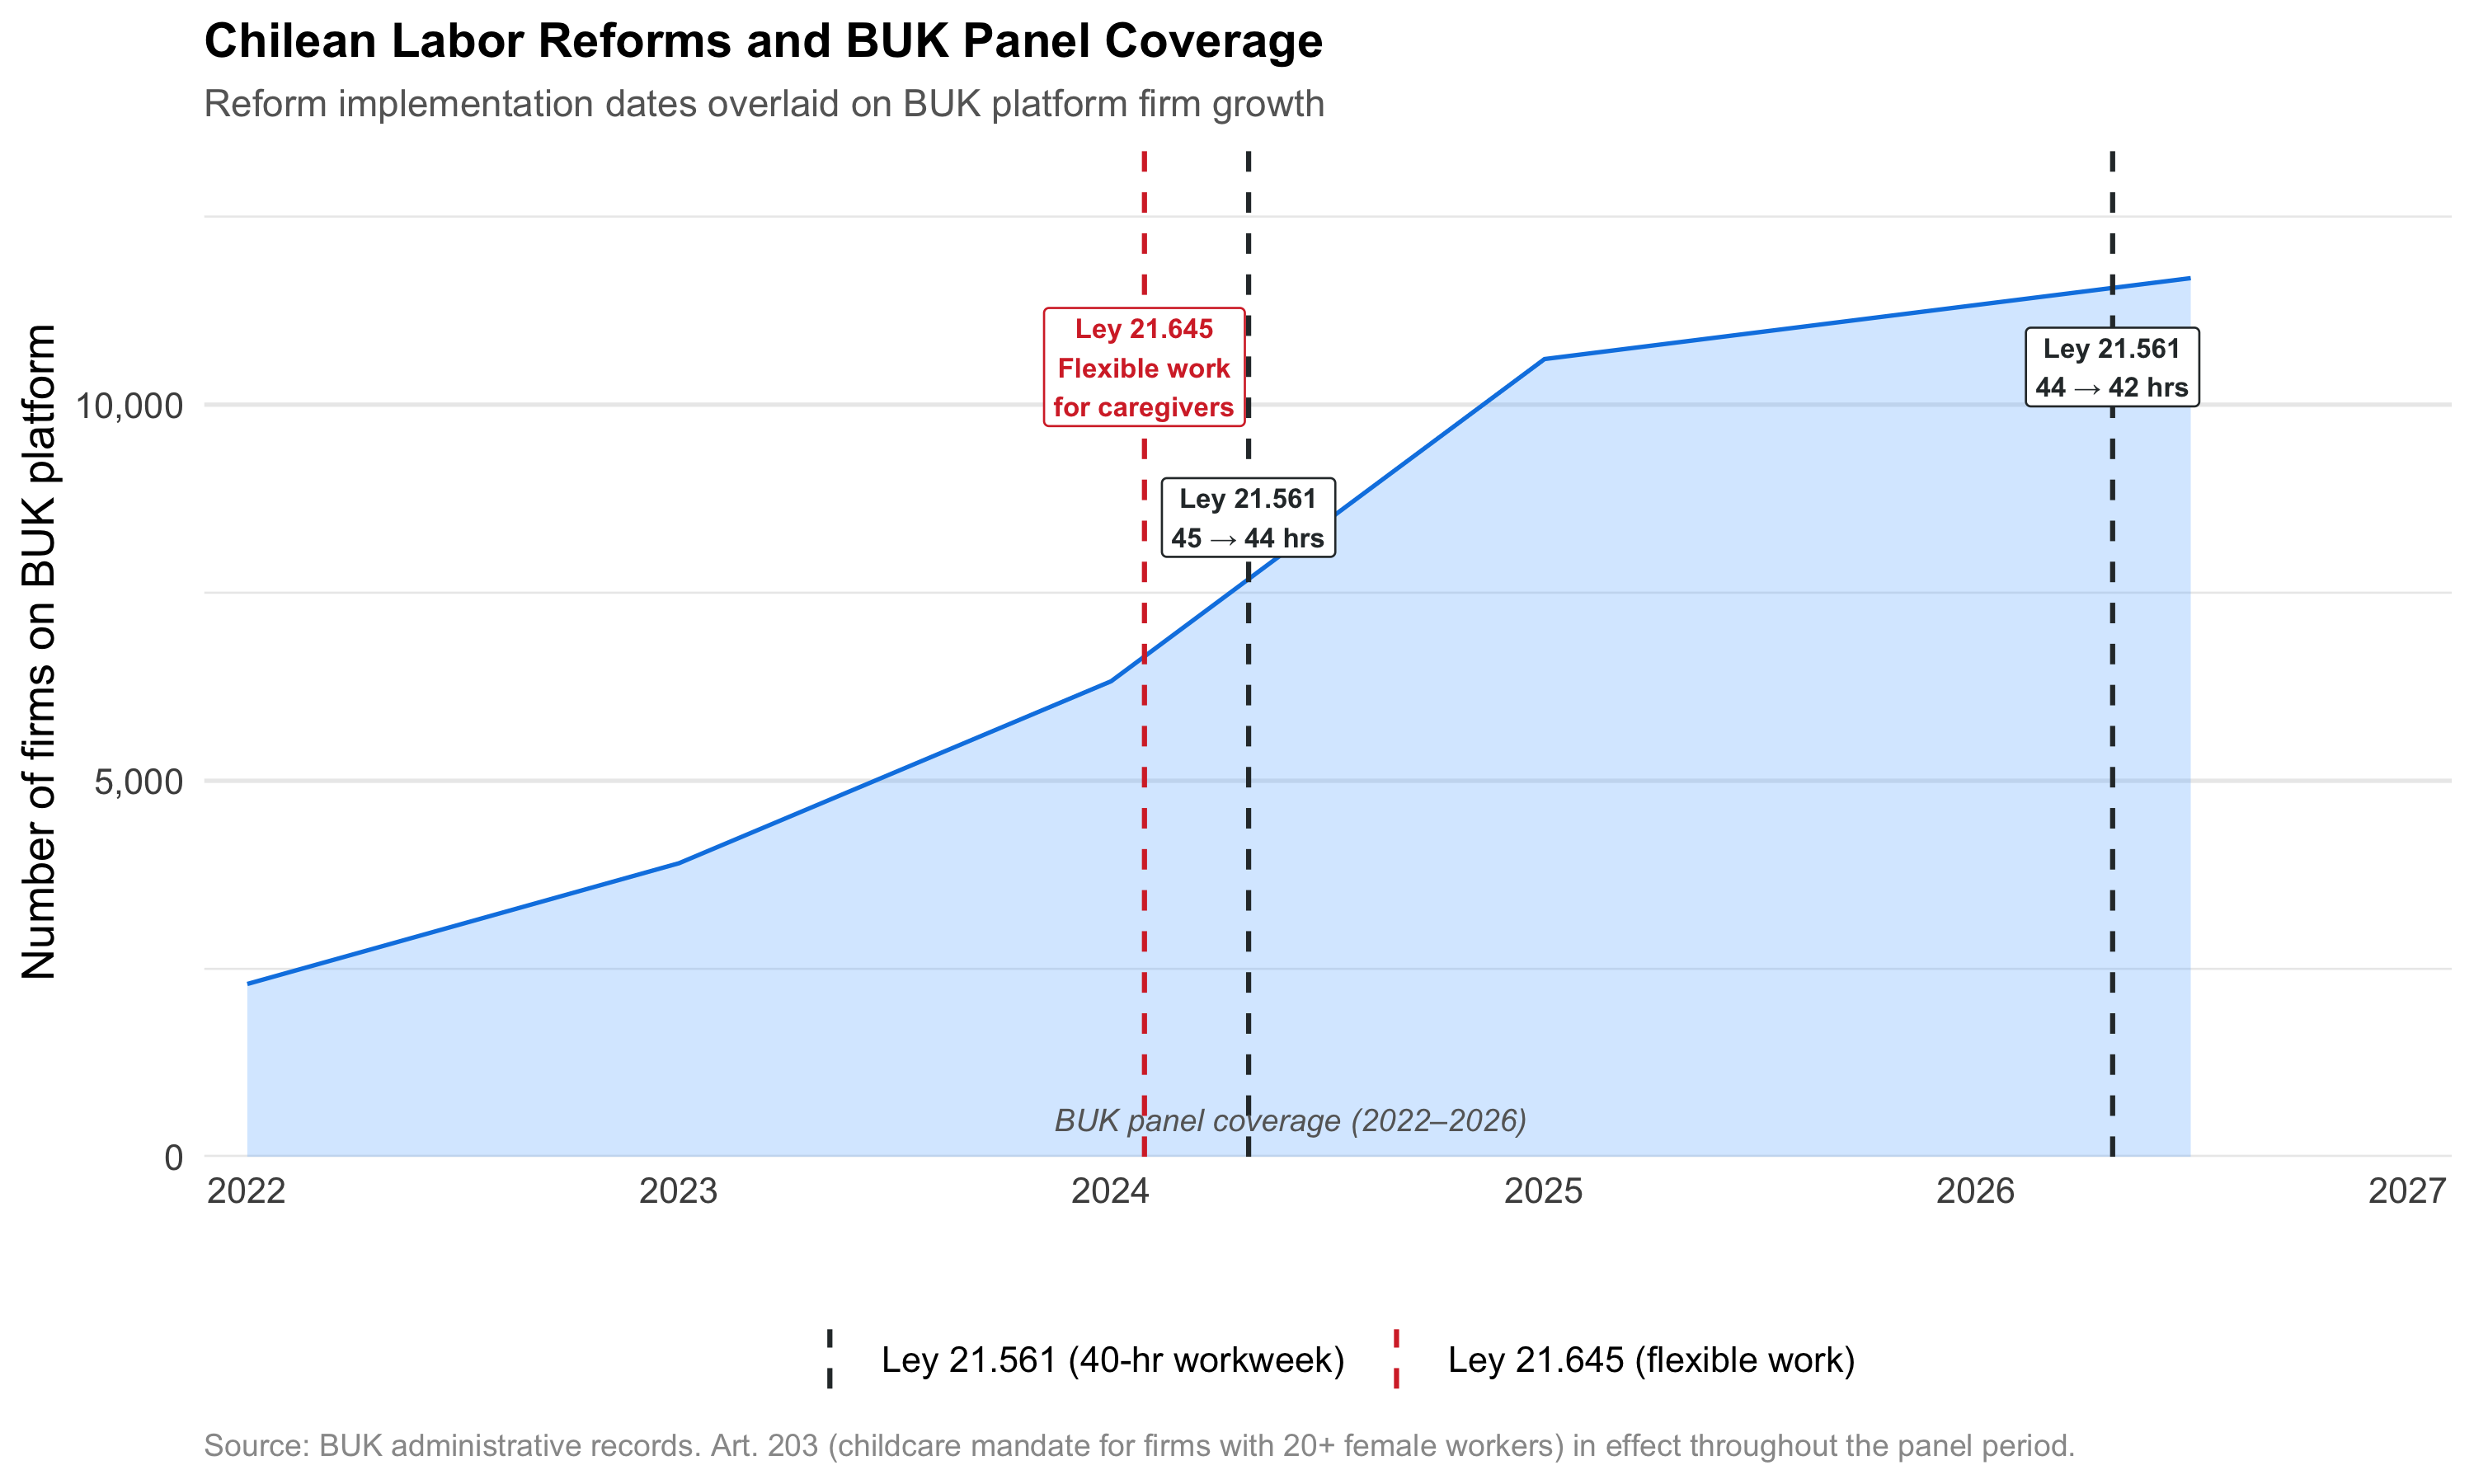
\includegraphics[width=0.60\textwidth]{rf_6_4_reform_timeline.png}
\end{center}

\vspace{-0.2cm}
\small
\begin{itemize}\itemsep1pt
    \item Platform grew from $\sim$6,500 firms (2022) to 19,000+ (2026); rapid adoption, not firm entry
    \item Three reforms fall \textbf{within the panel window}, creating pre/post variation
    \item Art.\ 203 childcare mandate in effect throughout --- cross-sectional RD at 20-female-worker threshold
\end{itemize}

\end{frame}

% --- Summary statistics: Firms ---
\begin{frame}
\frametitle{Firms: 19,000+ Chilean firms, skewed toward large employers}

\begin{center}
\small
\begin{tabular}{@{}lrr@{}}
\toprule
& \textbf{N firms} & \textbf{\% of workers} \\
\midrule
Large ($>$250 employees) & 5,459 \;\;(28.4\%) & 79.8\% \\
Medium (50--250) & 6,127 \;\;(31.9\%) & 14.5\% \\
Small ($<$50) & 7,612 \;\;(39.6\%) & 5.7\% \\
\midrule
\textbf{Total} & \textbf{19,358} & \textbf{100\%} \\
\bottomrule
\end{tabular}
\end{center}

\vspace{0.3cm}
\begin{itemize}
    \item 20 SII economic sectors represented; top 5: retail, professional services, admin services, finance, manufacturing
    \item Linkable to SII tax records for 87\% of firms (sector, sales bracket, equity range)
    \item Firm identifiers allow linking across all tables (workforce, salary, assignments, recruitment)
\end{itemize}

\end{frame}

% --- Summary statistics: Workers & Jobs ---
\begin{frame}
\frametitle{Workers: 4.7M employees with detailed job spells}

\begin{center}
\small
\begin{tabular}{@{}lr@{}}
\toprule
Unique workers & 4,712,667 \\
Job spells & 8,273,604 \\
Male / Female & 62.8\% / 37.2\% \\
\midrule
\multicolumn{2}{@{}l}{\textit{Job spells per worker}} \\[2pt]
Mean   & 5.86 \\
Median & 3.00 \\
P10 / P90 & 1.00 / 14.00 \\
\bottomrule
\end{tabular}
\end{center}

\vspace{0.3cm}
\begin{itemize}
    \item \textbf{Hierarchy:} supervisor identifier (\texttt{boss\_id}) enables org structure and promotion measurement
    \item \textbf{Job characteristics:} area, standardized occupation (CIUO-08 crosswalk), contract type (fixed-term / indefinite), workday type (full-time, part-time, Art.\ 22 exempt)
    \item \textbf{Separations:} end date for 83.2\% of completed spells; exit reason (voluntary / involuntary)
\end{itemize}

\end{frame}

% --- Summary statistics: Compensation ---
\begin{frame}
\frametitle{Compensation: monthly payroll and individual bonus assignments}

Two complementary tables allow decomposition of total compensation:

\vspace{0.3cm}
\begin{itemize}
    \item \textbf{Monthly payroll} (\texttt{adm\_salary}): base, gross, and net salary for each worker-month
    \begin{itemize}
        \item Taxable and non-taxable earnings observed separately
        \item Liquidation type distinguishes regular salary, severance (\textit{finiquito}), vacation pay, and bonuses
        \item Allows fixed vs.\ variable compensation decomposition
    \end{itemize}

    \medskip
    \item \textbf{Bonus assignments} (\texttt{adm\_assign}): individual assignment-level records
    \begin{itemize}
        \item Categories: performance bonus, tenure bonus, commission, \textit{aguinaldo}, transportation, meal allowance
        \item Each record has start/end dates and monetary amount
        \item Tracks whether the firm rewards through \emph{promotions} (title + base wage) or \emph{bonuses} (variable pay without advancement)
    \end{itemize}
\end{itemize}

\end{frame}

% --- Summary statistics: Recruitment ---
\begin{frame}
\frametitle{Recruitment: 186K hiring processes with application-level data}

\begin{center}
\small
\begin{tabular}{@{}lr@{}}
\toprule
Selection processes & 186,457 \\
Applications & 2,725,982 \\
Unique candidates & 839,664 \\
\midrule
Median apps per vacancy & 2 \\
Mean apps per vacancy & 18.7 \\
P90 apps per vacancy & 42 \\
\midrule
Candidate gender: Male / Female & 56.0\% / 43.0\% \\
\bottomrule
\end{tabular}
\end{center}

\vspace{0.3cm}
\begin{itemize}
    \item Each vacancy records functional area, salary range offered, and reason (new position, replacement, temporary)
    \item Each application has candidate demographics, referral source (portals 40.5\%, company 23.7\%, job boards 14.7\%), and application score
    \item Heavy right tail --- some vacancies attract 1,000+ applicants
\end{itemize}

\end{frame}

% ============================================================
% SECTION C: Sample Selection
% ============================================================

% --- BUK vs SII comparison ---
\begin{frame}
\frametitle{Sample selection: BUK vs.\ the universe of formal Chilean firms}

\begin{center}
\small
\begin{tabular}{@{}lrrrr@{}}
\toprule
 & \multicolumn{2}{c}{\textbf{Firms (\%)}} & \multicolumn{2}{c}{\textbf{Workers (\%)}} \\
\cmidrule(lr){2-3} \cmidrule(lr){4-5}
Size & BUK & SII & BUK & SII \\
\midrule
Micro/Small  & 39.6 & 95.3 & 5.7  & 29.9 \\
Medium       & 31.9 &  3.2 & 14.5 & 16.5 \\
Large        & 28.5 &  1.5 & 79.8 & 53.6 \\
\bottomrule
\end{tabular}
\end{center}

\vspace{0.2cm}
\begin{itemize}
    \item Large firms over-represented --- but this is an \textbf{advantage}: model predictions on hiring screening and promotion thresholds are most testable in firms with structured pipelines

    \medskip
    \item \textbf{Gender:} BUK sample is 37.2\% female; formal employment is $\sim$42\% female --- modest under-representation

    \medskip
    \item \textbf{Sectors:} public administration absent (public employers don't use platform); manufacturing under-represented; finance, education, real estate over-represented
\end{itemize}

\end{frame}

% --- Coverage heatmap ---
\begin{frame}
\frametitle{Coverage varies by sector and firm size}

\vspace{-0.1cm}
\begin{columns}[T]
\begin{column}{0.52\textwidth}
\includegraphics[width=\textwidth]{../../../../4_Code/images/heatmap_coverage.png}
\end{column}
\begin{column}{0.45\textwidth}
\small
\vspace{0.3cm}
Coverage rate = BUK firms / SII firms, by ISIC sector $\times$ firm size.

\vspace{0.3cm}
\begin{itemize}\itemsep4pt
    \item Strong coverage among \textbf{large firms} (30--46\%)
    \item Thin in micro/small and public administration
    \item Platform expanding into smaller firms (avg.\ empl./firm: 257 in 2022 $\to$ 166 in 2026)
\end{itemize}
\end{column}
\end{columns}

\end{frame}

% ============================================================
% SECTION D: Research Directions
% ============================================================

% --- Full menu ---
\begin{frame}
\frametitle{Many possible research questions}

\small
\begin{enumerate}\itemsep4pt
    \item \textbf{Monopsony power and career dynamics}
    \begin{itemize}
        \item Do firms with greater market power have larger gender gaps in promotions and hiring screening?
    \end{itemize}

    \item \textbf{Bonuses vs.\ promotions as retention tools}
    \begin{itemize}
        \item Do firms substitute variable pay (performance bonuses, commissions) for career advancement, especially for women?
    \end{itemize}

    \item \textbf{The 40-hour workweek and flexible schedule workers}
    \begin{itemize}
        \item Does restricting Art.\ 22 exemptions hurt workers who valued schedule flexibility --- particularly mothers?
    \end{itemize}

    \item \textbf{The broken rung at first promotion}
    \begin{itemize}
        \item Is there a gender gap at the first promotion, and do long-hours norms explain who gets promoted?
    \end{itemize}

    \item \textbf{Wage growth over the life cycle}
    \begin{itemize}
        \item How does market power shape wage trajectories by gender at different career stages?
    \end{itemize}
\end{enumerate}

\end{frame}

% --- Highlighted version ---
\begin{frame}
\frametitle{Many possible research questions}

\small
\begin{enumerate}\itemsep4pt
    \item \textbf{\textcolor{navy}{Monopsony power and career dynamics}}
    \begin{itemize}
        \item Do firms with greater market power have larger gender gaps in promotions and hiring screening?
    \end{itemize}

    \item \textcolor{faded}{Bonuses vs.\ promotions as retention tools}
    \begin{itemize}
        \item \textcolor{faded}{Do firms substitute variable pay (performance bonuses, commissions) for career advancement, especially for women?}
    \end{itemize}

    \item \textcolor{faded}{The 40-hour workweek and flexible schedule workers}
    \begin{itemize}
        \item \textcolor{faded}{Does restricting Art.\ 22 exemptions hurt workers who valued schedule flexibility --- particularly mothers?}
    \end{itemize}

    \item \textcolor{faded}{The broken rung at first promotion}
    \begin{itemize}
        \item \textcolor{faded}{Is there a gender gap at the first promotion, and do long-hours norms explain who gets promoted?}
    \end{itemize}

    \item \textcolor{faded}{Wage growth over the life cycle}
    \begin{itemize}
        \item \textcolor{faded}{How does market power shape wage trajectories by gender at different career stages?}
    \end{itemize}
\end{enumerate}

\end{frame}

% ============================================================
% SECTION E: Literature
% ============================================================

\begin{frame}
\frametitle{Three literatures have developed in parallel}

\small
\begin{itemize}\itemsep3pt
    \item \textbf{Imperfect competition in labor markets:} search frictions give firms market power (Manning, 2003); on-the-job search models show outside options shape the employment relationship (Burdett \& Mortensen, 1998; Postel-Vinay \& Robin, 2002); labor supply elasticities to firms are low (Sokolova \& Sorensen, 2021) --- \bmark{but the focus is on wages}

    \item \textbf{Outside options and gender:} women exhibit lower labor supply elasticities (Webber, 2016; Sharma, 2023); differences in outside options driven by commuting and mobility explain a meaningful share of the gender wage gap (Caldwell \& Danieli, 2022; Morchio \& Moser, 2024); women capture a smaller share of firm pay premiums (Card et al., 2016) --- \bmark{but still only studied for \emph{wages}}

    \item \textbf{Gender and career dynamics:} subjective ``potential'' assessments account for half the promotion gap (Benson et al., 2026); employers screen applicants differently by gender (Bertrand \& Mullainathan, 2004; Kline et al., 2022) --- \bmark{but no connection to \emph{market structure}}

    \item \textbf{This paper:} connects imperfect competition to gender gaps in career dynamics at both hiring and promotion margins
\end{itemize}

\end{frame}

% ============================================================
% SECTION F: Model
% ============================================================

% --- Model overview (intuitive) ---
\begin{frame}
\frametitle{Model: on-the-job search with hiring and promotion}

\textbf{Building on:} Burdett \& Mortensen (1998), extended with promotion decisions (Gibbons \& Waldman, 1999) and gender-specific outside options (Sharma, 2023).

\begin{center}
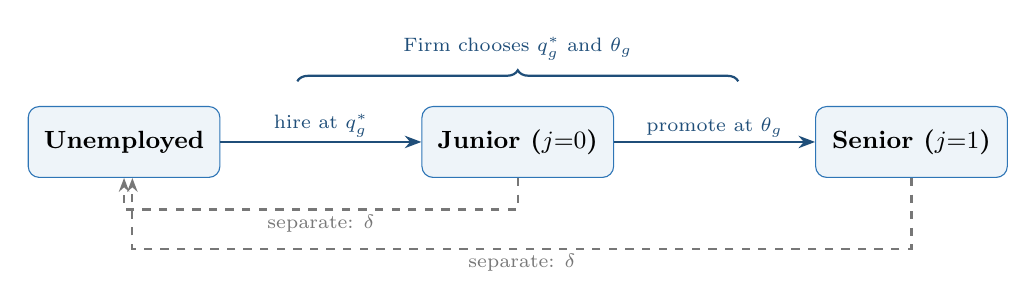
\begin{tikzpicture}[
  state/.style={draw=accentblue, rounded corners=4pt, fill=accentblue!8,
                text width=2.2cm, align=center, minimum height=0.9cm, font=\small\bfseries},
  firm/.style={-{Stealth[length=6pt]}, thick, navy},
  sep/.style={-{Stealth[length=5pt]}, thick, muted, dashed},
  lbl/.style={font=\scriptsize, fill=white, inner sep=1.5pt}]
  \node[state] (unemp) at (0,0) {Unemployed};
  \node[state] (junior) at (5,0) {Junior ($j{=}0$)};
  \node[state] (senior) at (10,0) {Senior ($j{=}1$)};
  \draw[firm] (unemp) -- (junior) node[lbl, midway, above] {hire at $q_g^*$};
  \draw[firm] (junior) -- (senior) node[lbl, midway, above] {promote at $\theta_g$};
  \draw[sep] (junior.south) -- ++(0,-0.4) -| (unemp.south)
    node[lbl, pos=0.25, below] {separate: $\delta$};
  \draw[sep] (senior.south) -- ++(0,-0.9) -| ([xshift=3pt]unemp.south)
    node[lbl, pos=0.25, below] {separate: $\delta$};
  \draw[navy, thick, decorate, decoration={brace, amplitude=4pt, raise=2pt}]
    (2.2,0.7) -- (7.8,0.7) node[midway, above=6pt, font=\scriptsize\color{navy}] {Firm chooses $q_g^*$ and $\theta_g$};
\end{tikzpicture}
\end{center}

\small
\begin{itemize}
    \item Two worker types ($g \in \{M, F\}$), firms with two job levels. Production is \textbf{gender-neutral} --- gender enters entirely through outside options
    \item \textbf{Key parameter:} outside offer arrival rate $\lambda_g$, with $\lambda_F < \lambda_M$
    \item Firms choose a \textbf{screening threshold} at hiring and a \textbf{promotion threshold} --- both shape careers
\end{itemize}
\hfill\hyperlink{model-formal}{\beamergotobutton{Formal model}}

\end{frame}

% --- Promotion mechanism (retention trade-off) ---
\begin{frame}[label=retentionslide]
\frametitle{The promotion mechanism: why monopsony distorts promotions}

The firm's promotion decision balances \textbf{two forces}:

\vspace{0.1cm}
\begin{enumerate}
    \item \textbf{Direct profit effect:} promoting raises output ($a_1 > a_0$), but also raises the wage ($w_{g1} > w_{g0}$). This trade-off is gender-neutral.
    \bigskip
    \item \textbf{Retention effect:} promoting makes the worker less likely to leave. This benefit depends on $\lambda_g$:
\end{enumerate}

\vspace{0.1cm}
\begin{columns}[T]
    \begin{column}{0.45\textwidth}
        \textbf{Men} (high $\lambda_M$):
        \begin{itemize}
            \item ``If I don't promote him, he'll leave''
            \item Retention urgency is \textbf{high}
            \item[$\Rightarrow$] Promote to retain
        \end{itemize}
    \end{column}
    \begin{column}{0.45\textwidth}
        \textbf{Women} (low $\lambda_F$):
        \begin{itemize}
            \item ``Even without promotion, she won't leave''
            \item Retention urgency is \textbf{low}
            \item[$\Rightarrow$] Delay is low-cost
        \end{itemize}
    \end{column}
\end{columns}

\vspace{0.3cm}
$\Rightarrow$ $\theta_F^* > \theta_M^*$: higher bar for women, not from productivity differences, but because firms face \textbf{less competitive pressure} to promote them.
\hfill\hyperlink{foc-formal}{\beamergotobutton{Formal FOC}}

\end{frame}

% --- Hiring mechanism ---
\begin{frame}
\frametitle{The hiring mechanism: why monopsony distorts screening}

When $\lambda_F < \lambda_M$, two \textbf{opposing forces} shape the firm's screening threshold $q_g^*$:

\vspace{0.3cm}
\begin{enumerate}
    \item \textbf{``Longer tenure'' force} $\to$ screen women \emph{less}

    Women stay longer at the firm $\to$ each hire generates surplus over more periods $\to$ the expected value of a marginal hire is higher $\to$ firm should lower the bar to hire more women

    \bigskip
    \item \textbf{``Less competition'' force} $\to$ screen women \emph{more}

    Women have fewer outside options $\to$ they apply even when the bar is high $\to$ firm can raise $q_F^*$ without losing its applicant pool $\to$ ``cherry-pick''
\end{enumerate}

\vspace{0.3cm}
\textbf{The sign of $q_F^* - q_M^*$ is ambiguous} --- which force dominates is an \textbf{empirical question}.

\vspace{0.2cm}
\textbf{Test:} BUK application-to-hire conversion rates by gender, across markets with different concentration.

\end{frame}

% ============================================================
% SECTION G: Preliminary Evidence
% ============================================================

% --- HHI distribution ---
\begin{frame}
\frametitle{Market concentration varies substantially across labor markets}

HHI computed over occupation $\times$ region cells (8 functional areas $\times$ 16 regions = 1,017 cells):

\vspace{-0.1cm}
\begin{center}
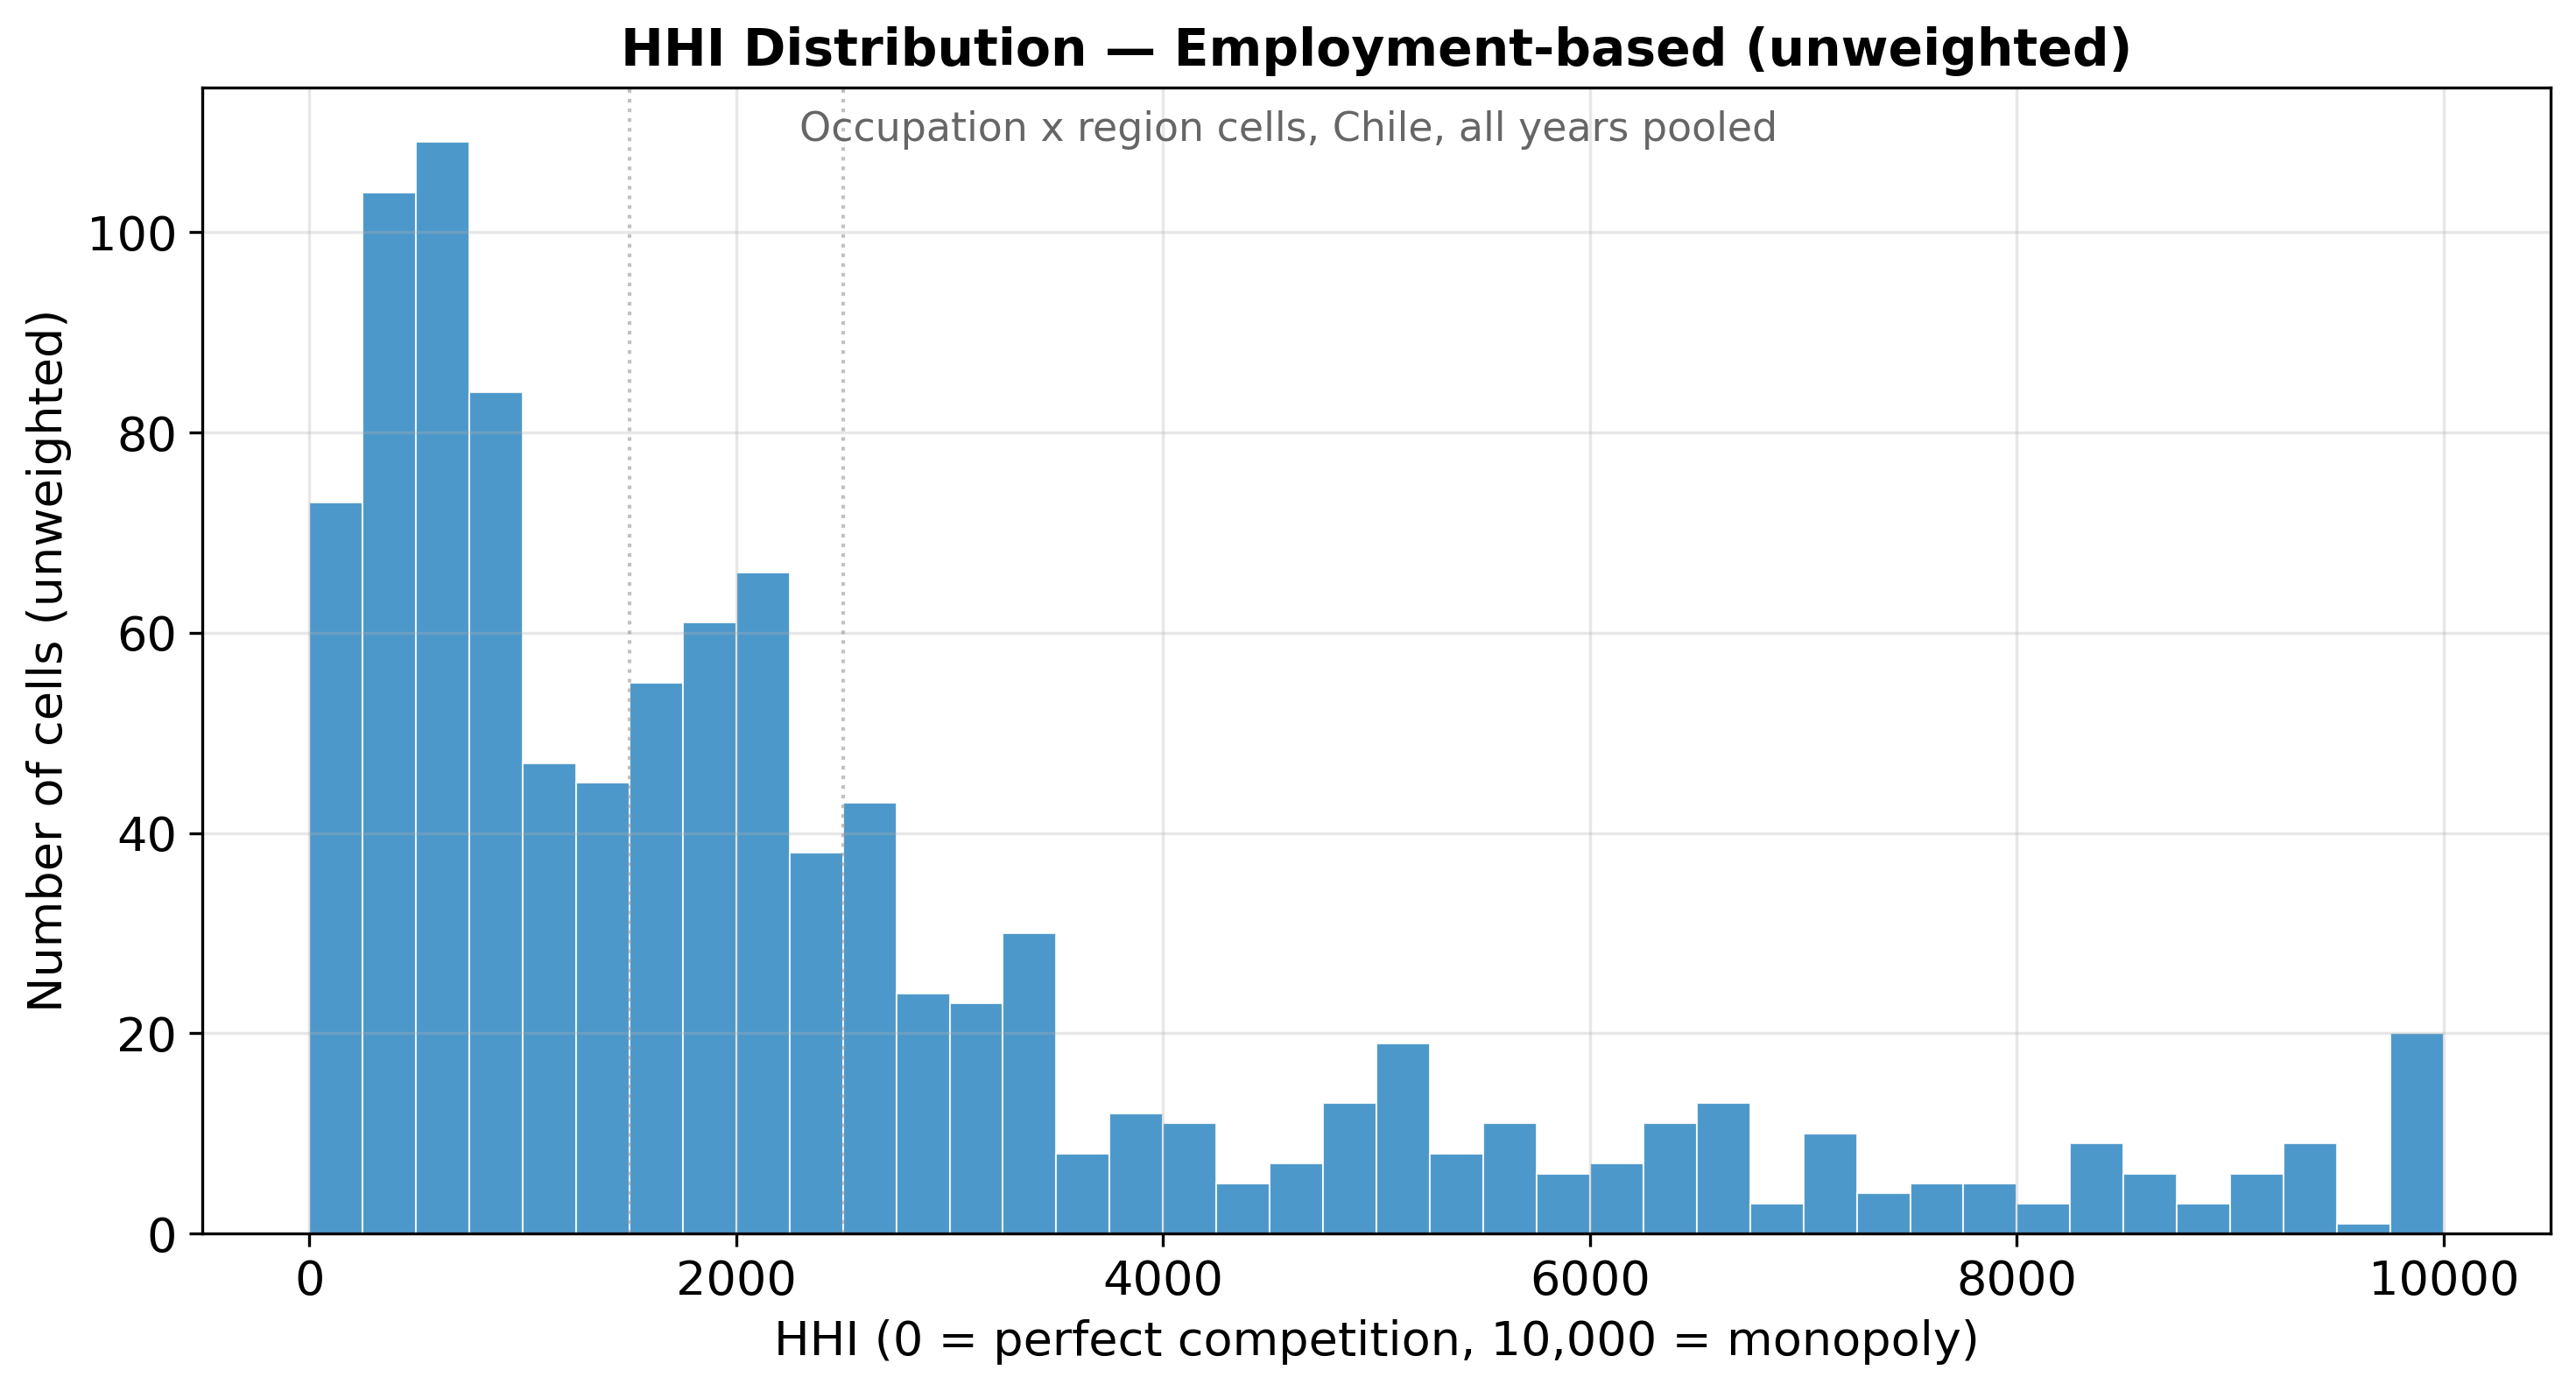
\includegraphics[width=0.58\textwidth]{rf_2_4_hhi_distribution_employment_unweighted.png}
\end{center}

\vspace{-0.2cm}
\small
\begin{itemize}\itemsep1pt
    \item Employment-based mean HHI = 2,249 (moderately concentrated), but substantial right tail
    \item Geographic variation: Santiago (HHI $\approx$ 209) vs.\ peripheral regions like Ays\'en (HHI $\approx$ 5,690)
    \item Vacancy-based HHI shows even higher concentration (mean 6,073), driven by thin markets
\end{itemize}

\end{frame}

% --- Promotion gap x concentration (KEY FIGURE) ---
\begin{frame}
\frametitle{The gender promotion gap reverses with market concentration}

\begin{center}
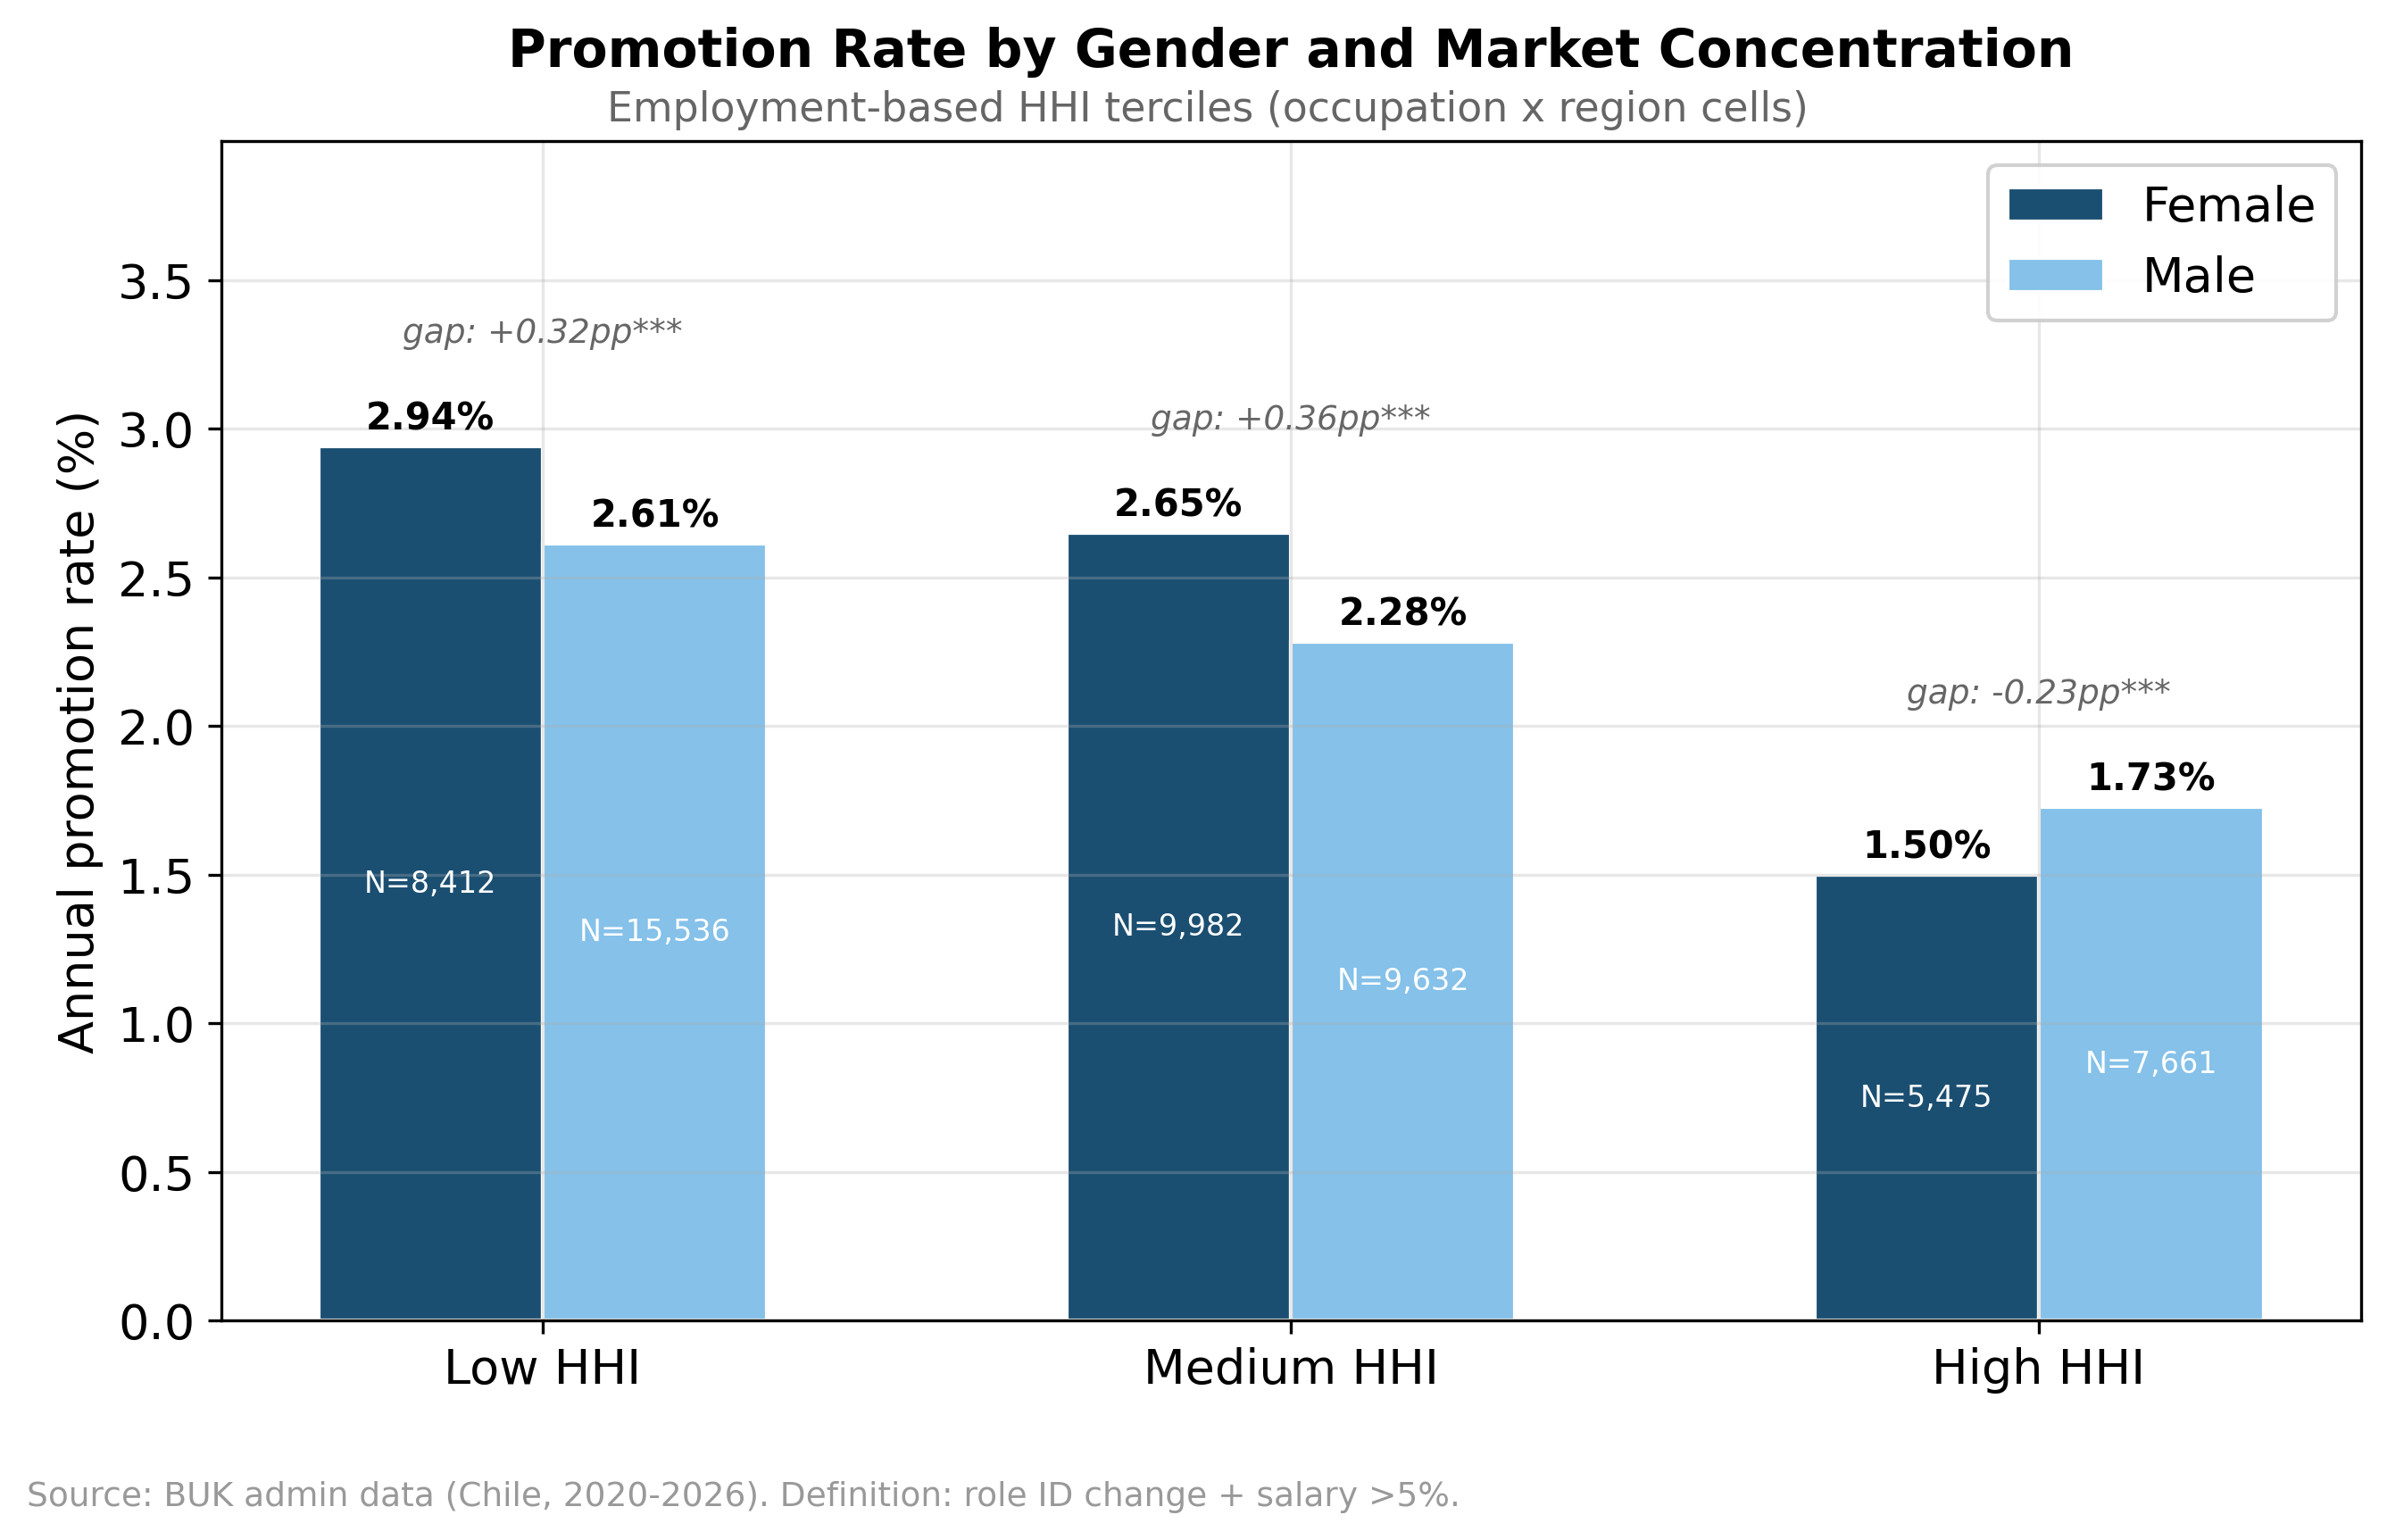
\includegraphics[width=0.62\textwidth]{rf_4_3_promotion_by_gender_hhi.png}
\end{center}

\vspace{-0.1cm}
\small
\begin{itemize}\itemsep2pt
    \item Aggregate promotion rates nearly identical (F: 2.10\%, M: 2.04\%; 73K promotions over 3.5M person-years)
    \item But \textbf{the gap reverses with concentration}: women promoted more in competitive markets (+0.32pp), less in concentrated markets ($-$0.23pp)
    \item Consistent with the retention mechanism: in concentrated markets, women's outside options are weakest, so firms can delay promotions at little cost
\end{itemize}

\end{frame}

% --- Survey evidence ---
\begin{frame}
\frametitle{Survey evidence: perceived inequity widens with organization size}

\begin{center}
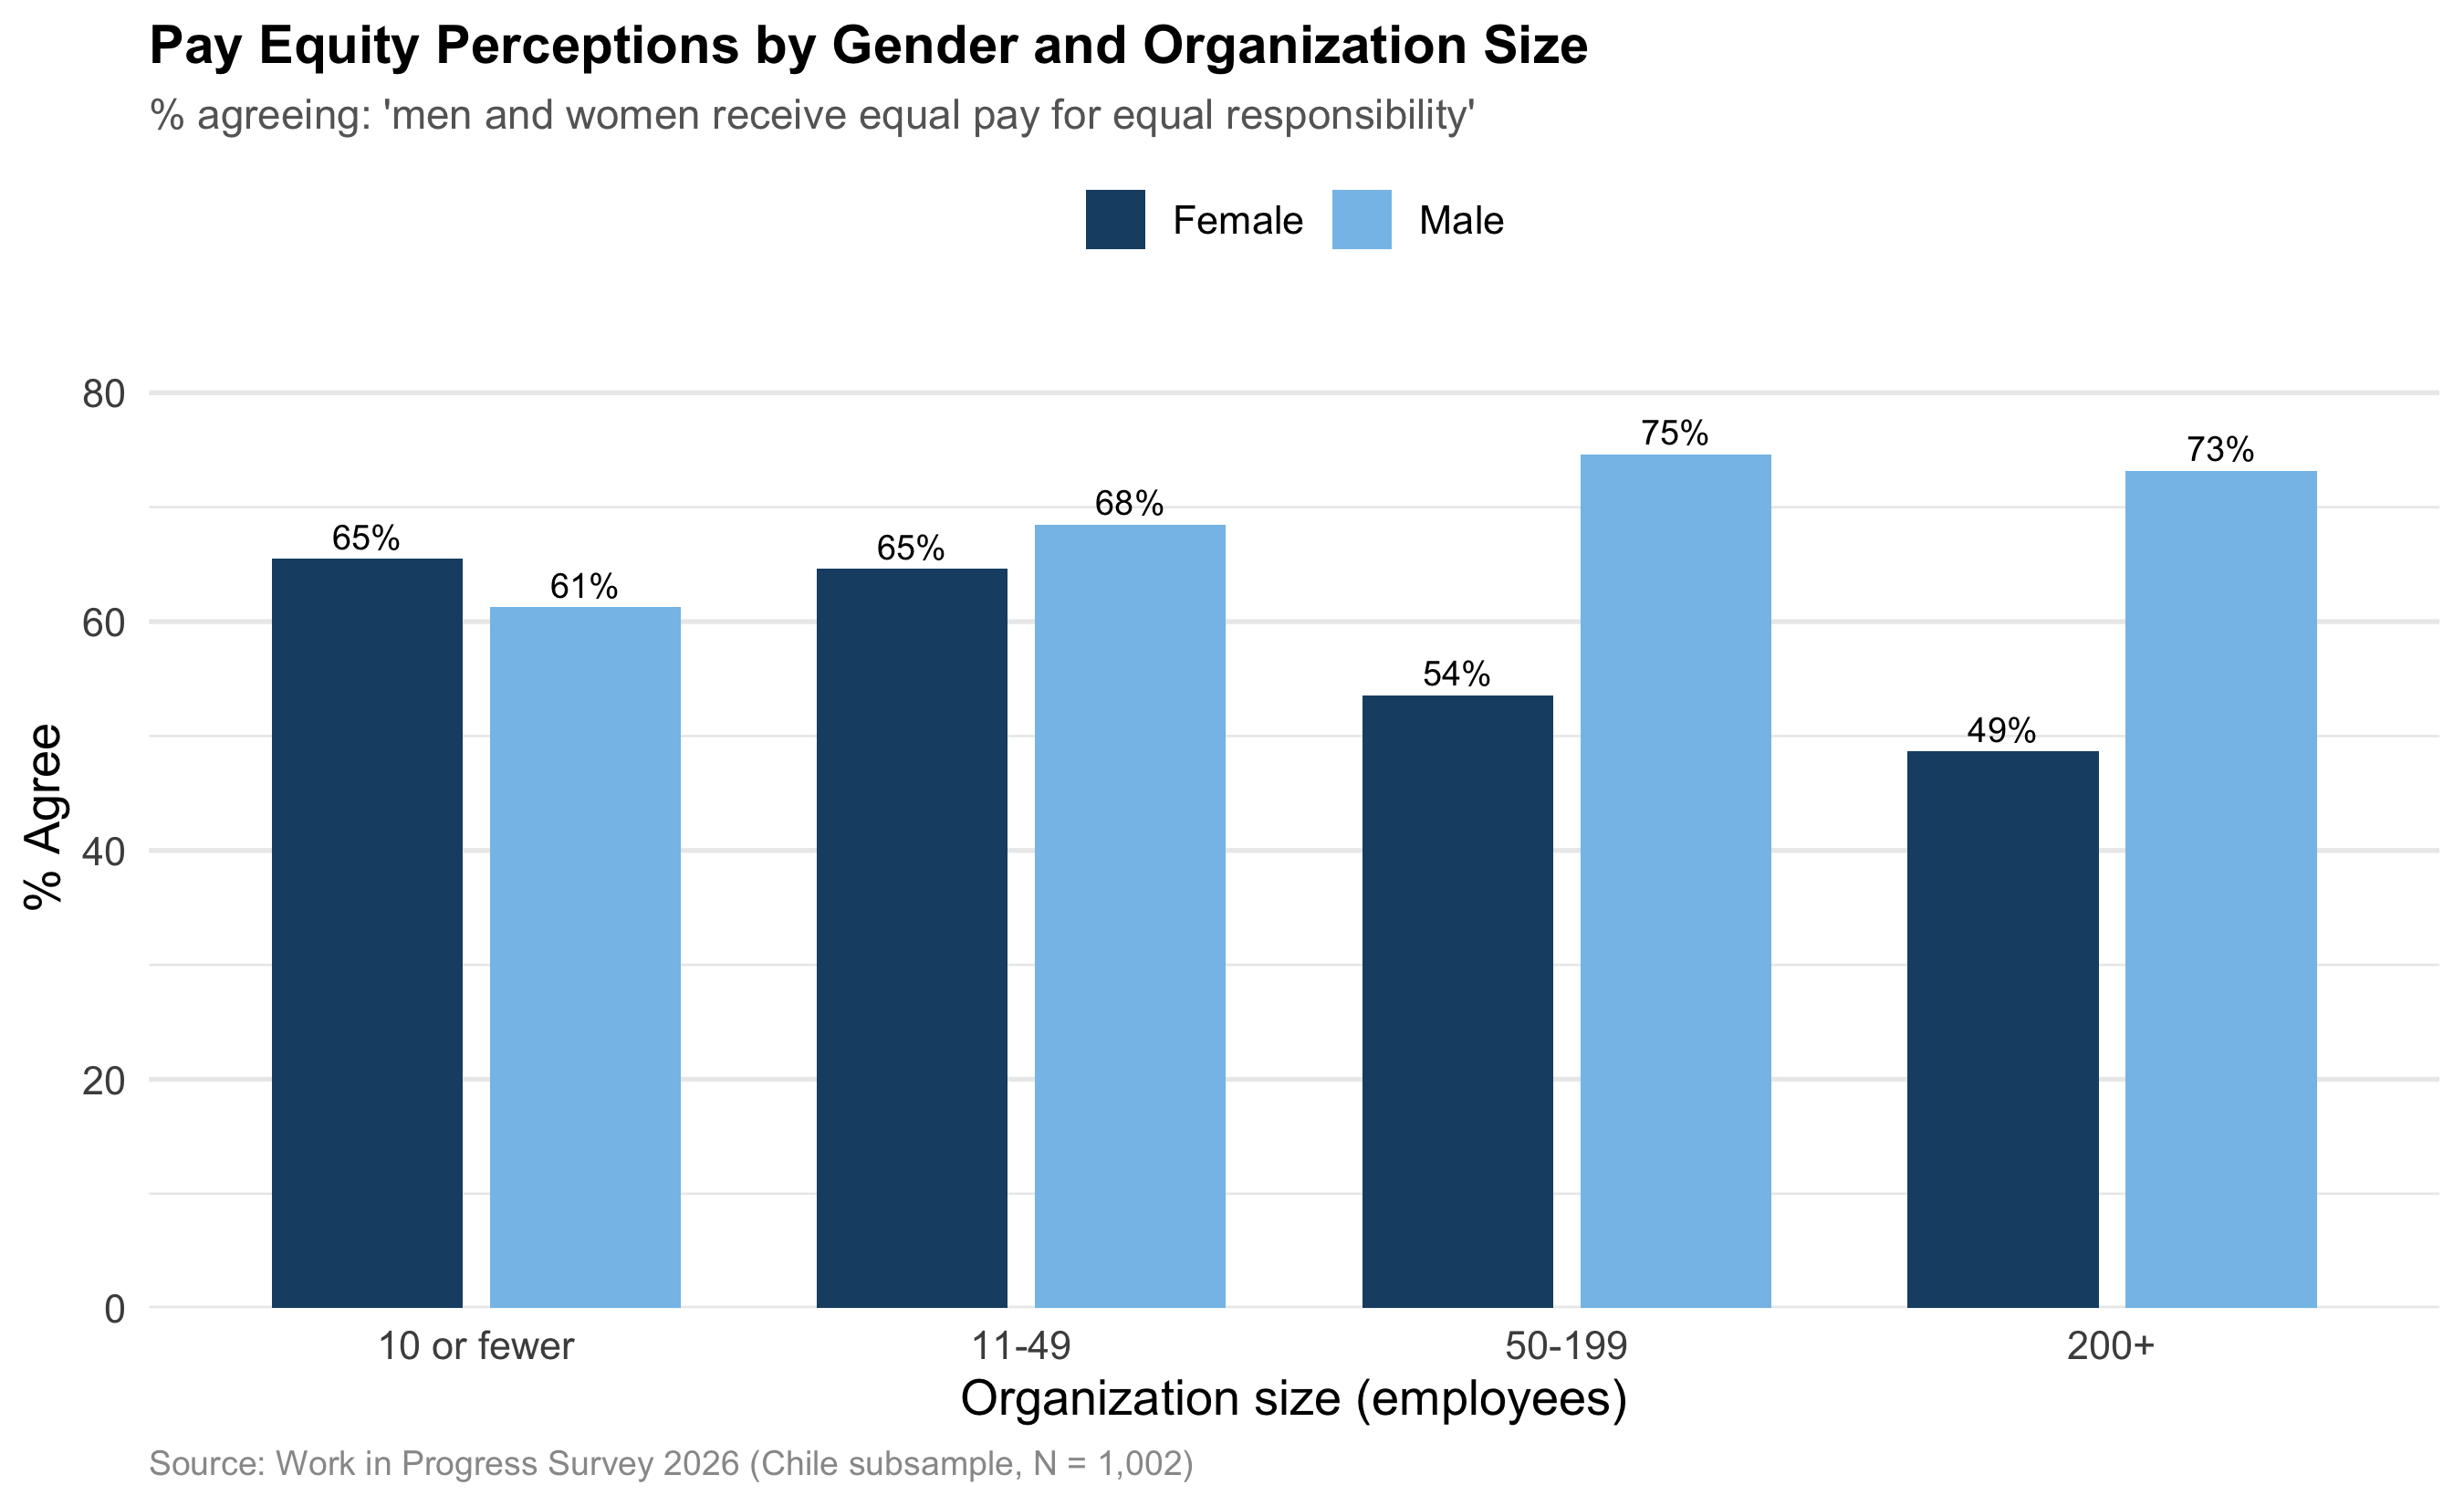
\includegraphics[width=0.55\textwidth]{rf_5_6_pay_equity_by_gender_x_orgsize.png}
\end{center}

\vspace{-0.2cm}
\small
\begin{itemize}\itemsep2pt
    \item Women perceive \textbf{less pay equity} than men, and the gap \textbf{widens with organization size} --- paralleling the HHI interaction in the promotion data
    \item Women report fewer promotion opportunities and face worse outcomes at every stage of salary negotiation (WiP Survey 2026)
    \item Lack of growth is the \textbf{top reason} workers of both genders cite for wanting to change jobs
\end{itemize}

\end{frame}

% --- Next steps ---
\begin{frame}
\frametitle{Remaining descriptive work and next steps}

Several pieces of evidence that would strengthen the case are still in progress:

\vspace{0.3cm}
\begin{itemize}
    \item \textbf{Job-to-job transition rates by gender} --- the most direct test of whether women face fewer outside options. Requires supplementary administrative records (unemployment insurance data)

    \medskip
    \item \textbf{Application-to-hire conversion rates by gender $\times$ HHI} --- tests the model's hiring prediction; the hired variable in the recruitment module is still being constructed

    \medskip
    \item \textbf{Wage growth at promotion by gender $\times$ HHI} --- tests whether the promotion gap translates into different wage trajectories

    \medskip
    \item \textbf{Structural labor supply elasticity estimates} --- complement HHI with estimates that distinguish vertical and horizontal sources of monopsony power (Sharma, 2023; Schubert et al., 2024)
\end{itemize}

\end{frame}

% ============================================================
% SECTION H: Counterfactuals
% ============================================================


% ============================================================
% APPENDIX
% ============================================================
\appendix
\setbeamertemplate{footline}{} % hide frame number in appendix

% --- Appendix: Formal model ---
\begin{frame}[label=model-formal]
\frametitle{Formal model: workers' problem}

\small
Workers of gender $g$ are either \textbf{unemployed} or \textbf{employed} at level $j \in \{0,1\}$ in a firm of type $p$.

\vspace{0.2cm}
\textbf{Value of unemployment:}
\begin{equation*}
    rU_g = b + \lambda_g^u \int \max\{V_{g0}(w) - U_g,\; 0\} \, dF_g(w)
\end{equation*}

\textbf{Value of employment at level $j$:}
\begin{align*}
    rV_{gj}(p) = & \; w_{gj}(p) + \lambda_g \int \max\{V_{g0}(w') - V_{gj}(p),\; 0\} \, dF_g(w') + \delta[U_g - V_{gj}(p)] \\
    & + \mathbbm{1}_{j=0} \cdot \mu_g(p)[V_{g1}(p) - V_{g0}(p)]
\end{align*}

\begin{itemize}
    \item $\lambda_g$: on-the-job outside offer arrival rate (\textbf{$\lambda_F < \lambda_M$})
    \item $\mu_g(p)$: promotion rate at firm $p$ for gender $g$ (determined by firm's choice)
\end{itemize}

\hfill\hyperlink{retentionslide}{\beamerreturnbutton{Back}}

\end{frame}

% --- Appendix: Firm's optimization ---
\begin{frame}
\frametitle{Formal model: firm's problem}

\small
The firm chooses $(w_{g0}, w_{g1}, q_g^*, \theta_g)$ to maximize steady-state profits:

\begin{equation*}
    \pi_g(p) = \sum_{j \in \{0,1\}} \bigl[y_{j}(p) - w_{gj}\bigr] \cdot n_{gj}(p)
\end{equation*}

where the steady-state workforce $n_{gj}(p)$ depends on three flows:

\vspace{0.2cm}
\begin{enumerate}
    \item \textbf{Inflow} (hiring): $h_g(p) = \lambda_g^u \cdot u_g \cdot [1 - H(q_g^*)] \cdot \mathbbm{1}\{V_{g0}(p) \geq U_g\}$
    \medskip
    \item \textbf{Internal flow} (promotion): $\mu_g(p) = 1 - G(\theta_g)$
    \medskip
    \item \textbf{Outflow} (separation): $s_g(p) = \delta + \lambda_g \cdot [1 - F_g(V_{gj}(p))]$
\end{enumerate}

\vspace{0.2cm}
In steady state:
\begin{align*}
    n_{g0}(p) &= \frac{h_g(p)}{\mu_g(p) + s_g(p)}, \qquad
    n_{g1}(p) = \frac{\mu_g(p) \cdot h_g(p)}{s_g(p) \cdot [\mu_g(p) + s_g(p)]}
\end{align*}

\hfill\hyperlink{retentionslide}{\beamerreturnbutton{Back}}

\end{frame}

% --- Appendix: Formal FOC ---
\begin{frame}[label=foc-formal]
\frametitle{Formal promotion condition (two-period simplification)}

\small
\textbf{Setup:} Period 1, worker is junior (profit $\pi_0 = pa_0 - w_{g0}$). Between periods, outside offer arrives with probability $\lambda_g$. If promoted, continuation value rises: $V_{1g} > V_{0g}$.

\vspace{0.1cm}
\textbf{Retention probabilities:}
\vspace{-0.1cm}
\begin{align*}
    r_g^P &= 1 - \lambda_g[1 - F_g(V_{1g})] \quad \text{(if promoted)} \\
    r_g^N &= 1 - \lambda_g[1 - F_g(V_{0g})] \quad \text{(if not promoted)}
\end{align*}

\vspace{-0.2cm}
Since $V_{1g} > V_{0g}$: $r_g^P > r_g^N$ (promoted workers are easier to retain).

\vspace{0.1cm}
\textbf{Promote if period-2 expected profit is higher with promotion:}
\begin{equation*}
    \underbrace{(\pi_1 - \pi_0) \cdot r_g^N}_{\substack{\text{Direct profit effect}}} + \underbrace{\pi_1 \cdot (r_g^P - r_g^N)}_{\substack{\text{Retention value} \\ \text{of promoting}}} \;\geq\; 0
\end{equation*}

\vspace{0.1cm}
\textbf{The retention term is proportional to $\lambda_g$:}
$\quad r_g^P - r_g^N = \lambda_g \bigl[F_g(V_{1g}) - F_g(V_{0g})\bigr]$

\vspace{0.1cm}
\begin{itemize}
    \item As $\lambda_g \to 0$: retention term vanishes $\to$ promote only if $\pi_1 > \pi_0$
    \item As $\lambda_g \to \infty$: retention dominates $\to$ always promote to retain
    \item Since $\lambda_F < \lambda_M$: retention motive is weaker for women $\to$ $\theta_F^* > \theta_M^*$
\end{itemize}

\hfill\hyperlink{retentionslide}{\beamerreturnbutton{Back}}

\end{frame}

% --- Appendix: Survey details ---
\begin{frame}[label=survey]
\frametitle{Work in Progress 2026 Survey}

\begin{itemize}
    \item \textbf{Sample:} 6,789 respondents in Chile, Colombia, Mexico, Peru
    \item \textbf{Open survey} --- anyone can respond; \textbf{cannot be linked} to platform data
    \item \textbf{Topics covered:}
    \begin{itemize}
        \item Demographics, salary, job tenure, firm size
        \item Job satisfaction, burnout, work-life balance
        \item Gender equity perceptions, discrimination, D\&I policies
        \item Benefits, performance evaluation, retention intentions
    \end{itemize}
    \item Provides \textbf{subjective} complement to BUK's \textbf{administrative} records
\end{itemize}

\vfill
{\scriptsize\textcolor{muted}{Source: BUK Work in Progress Survey 2026.}}
\hfill\hyperlink{bukslide}{\beamerreturnbutton{Back}}

\end{frame}

% --- Appendix: Additional figures ---
\begin{frame}
\frametitle{Gender composition of BUK firms by sector and size}

\begin{center}
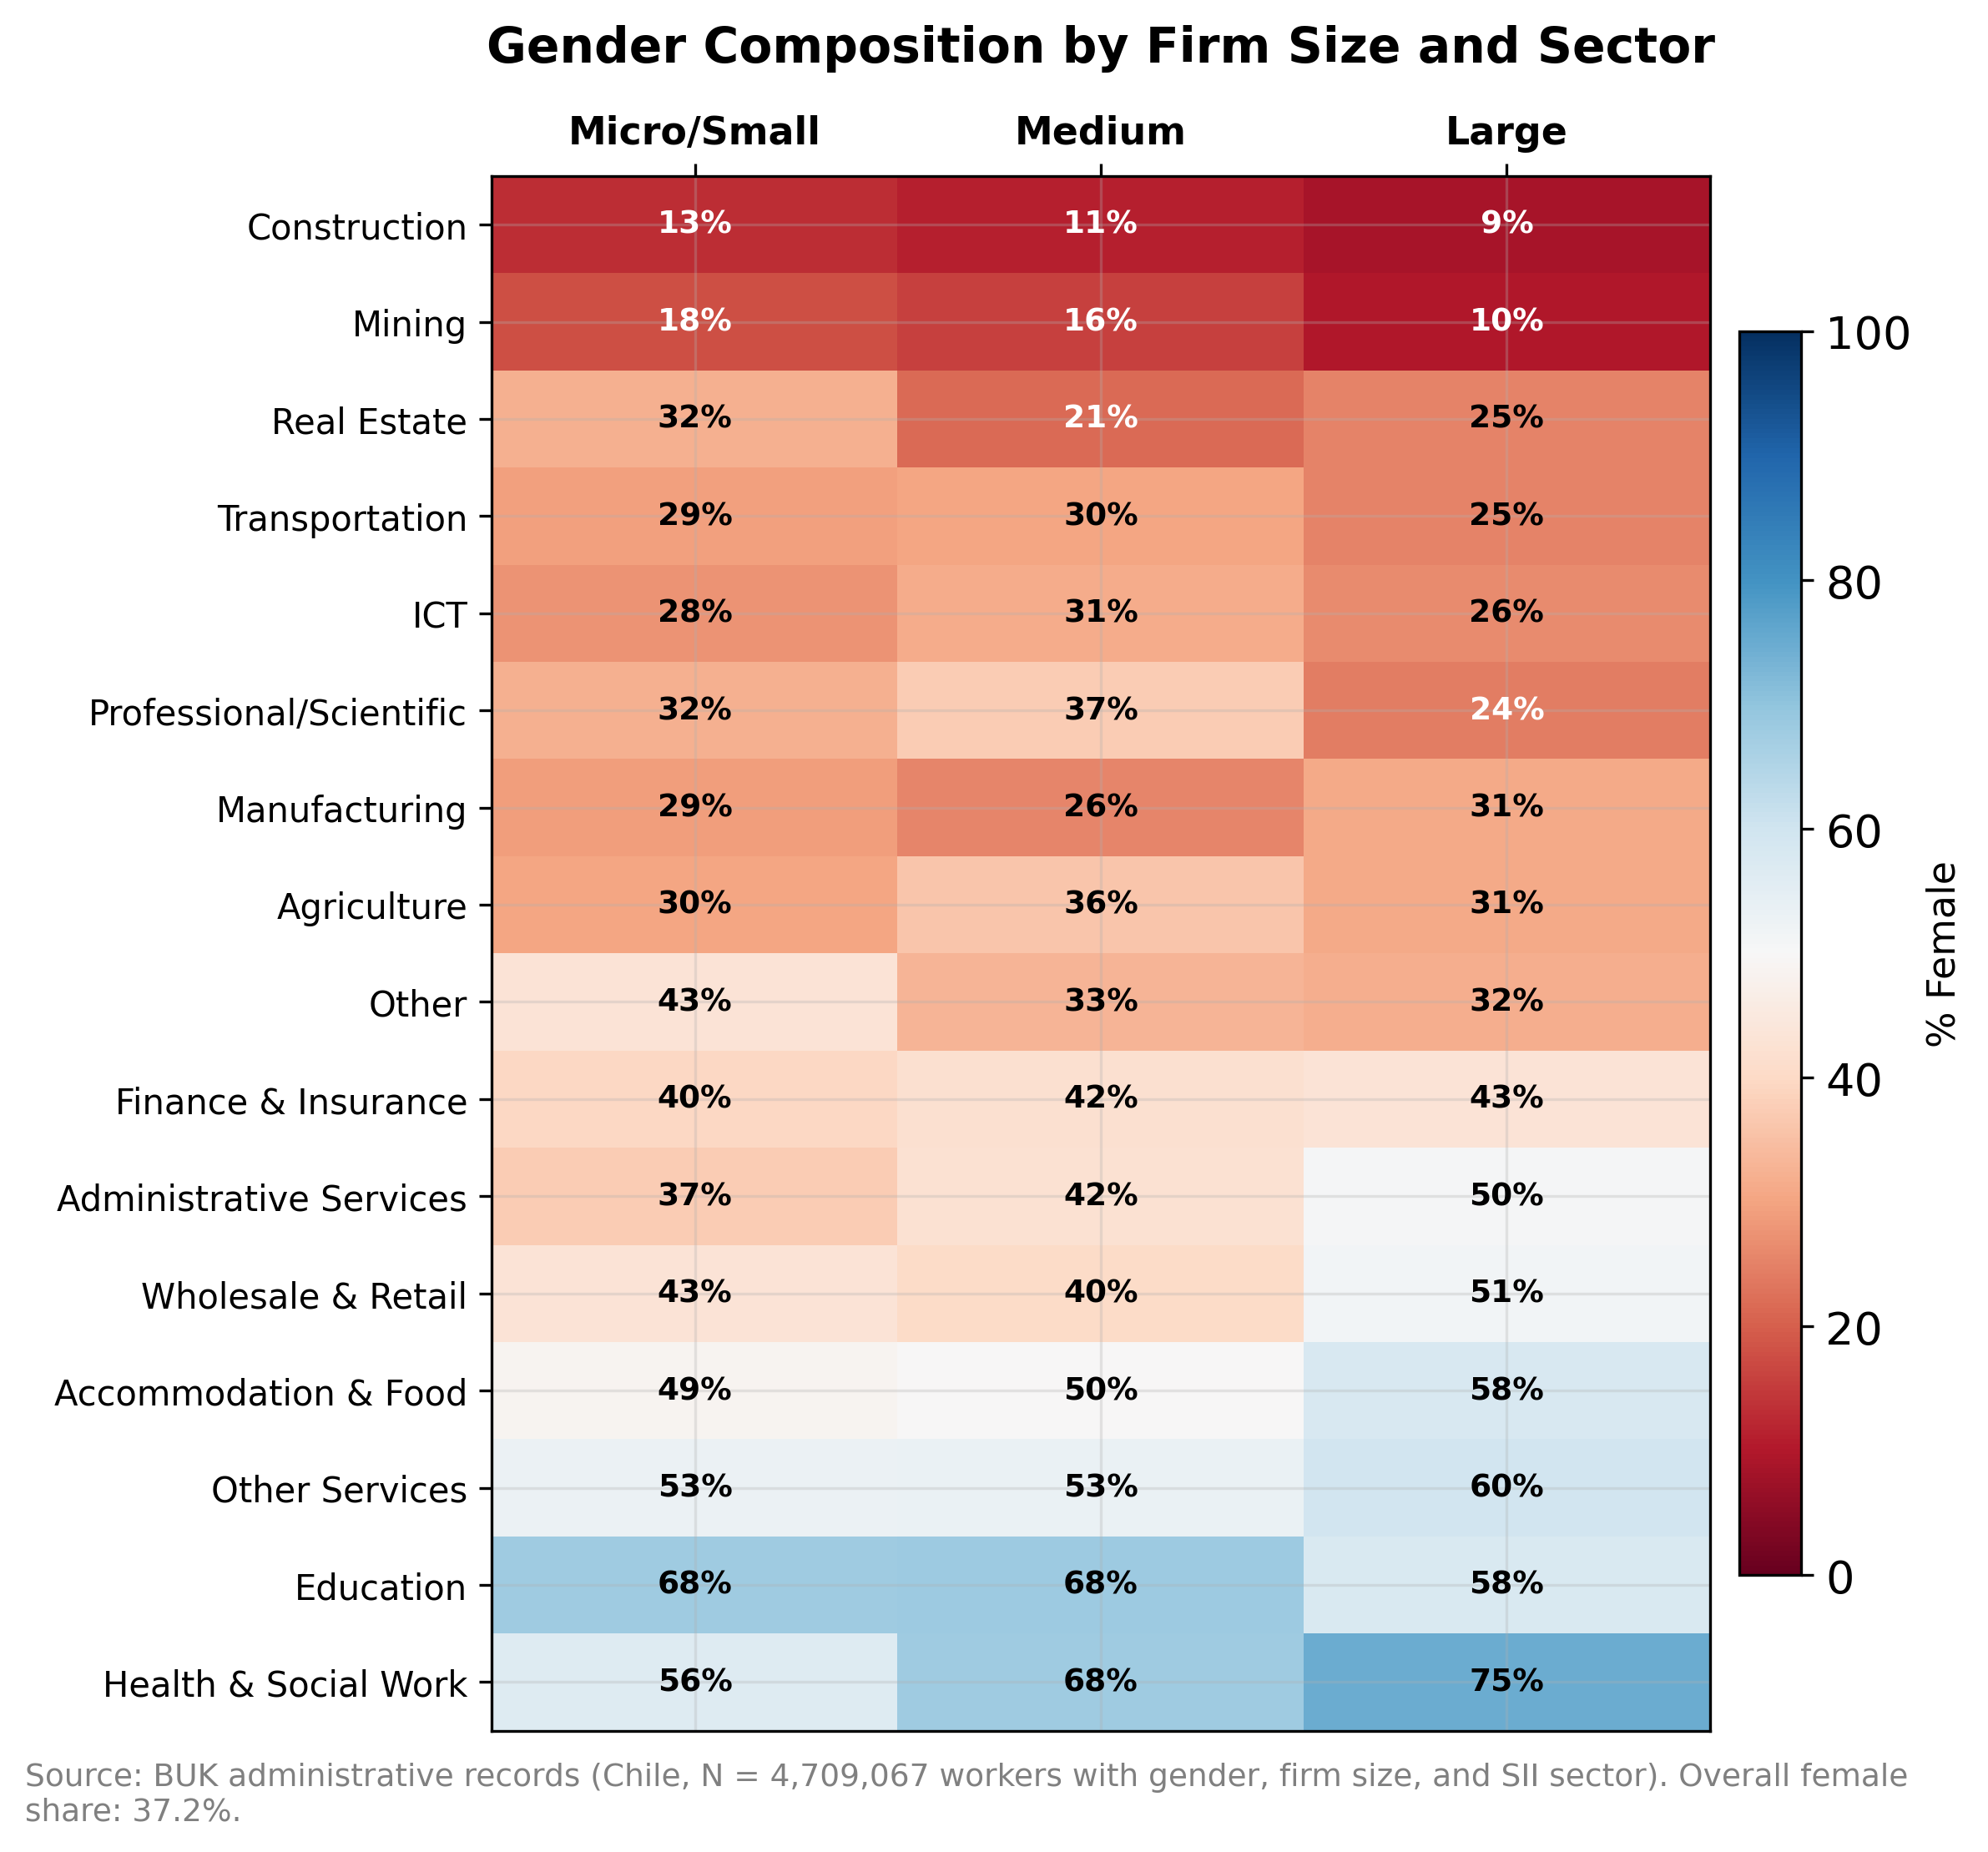
\includegraphics[width=0.72\textwidth]{rf_6_3_gender_composition.png}
\end{center}

\end{frame}

\begin{frame}
\frametitle{Salary negotiation funnel by gender}

\begin{center}
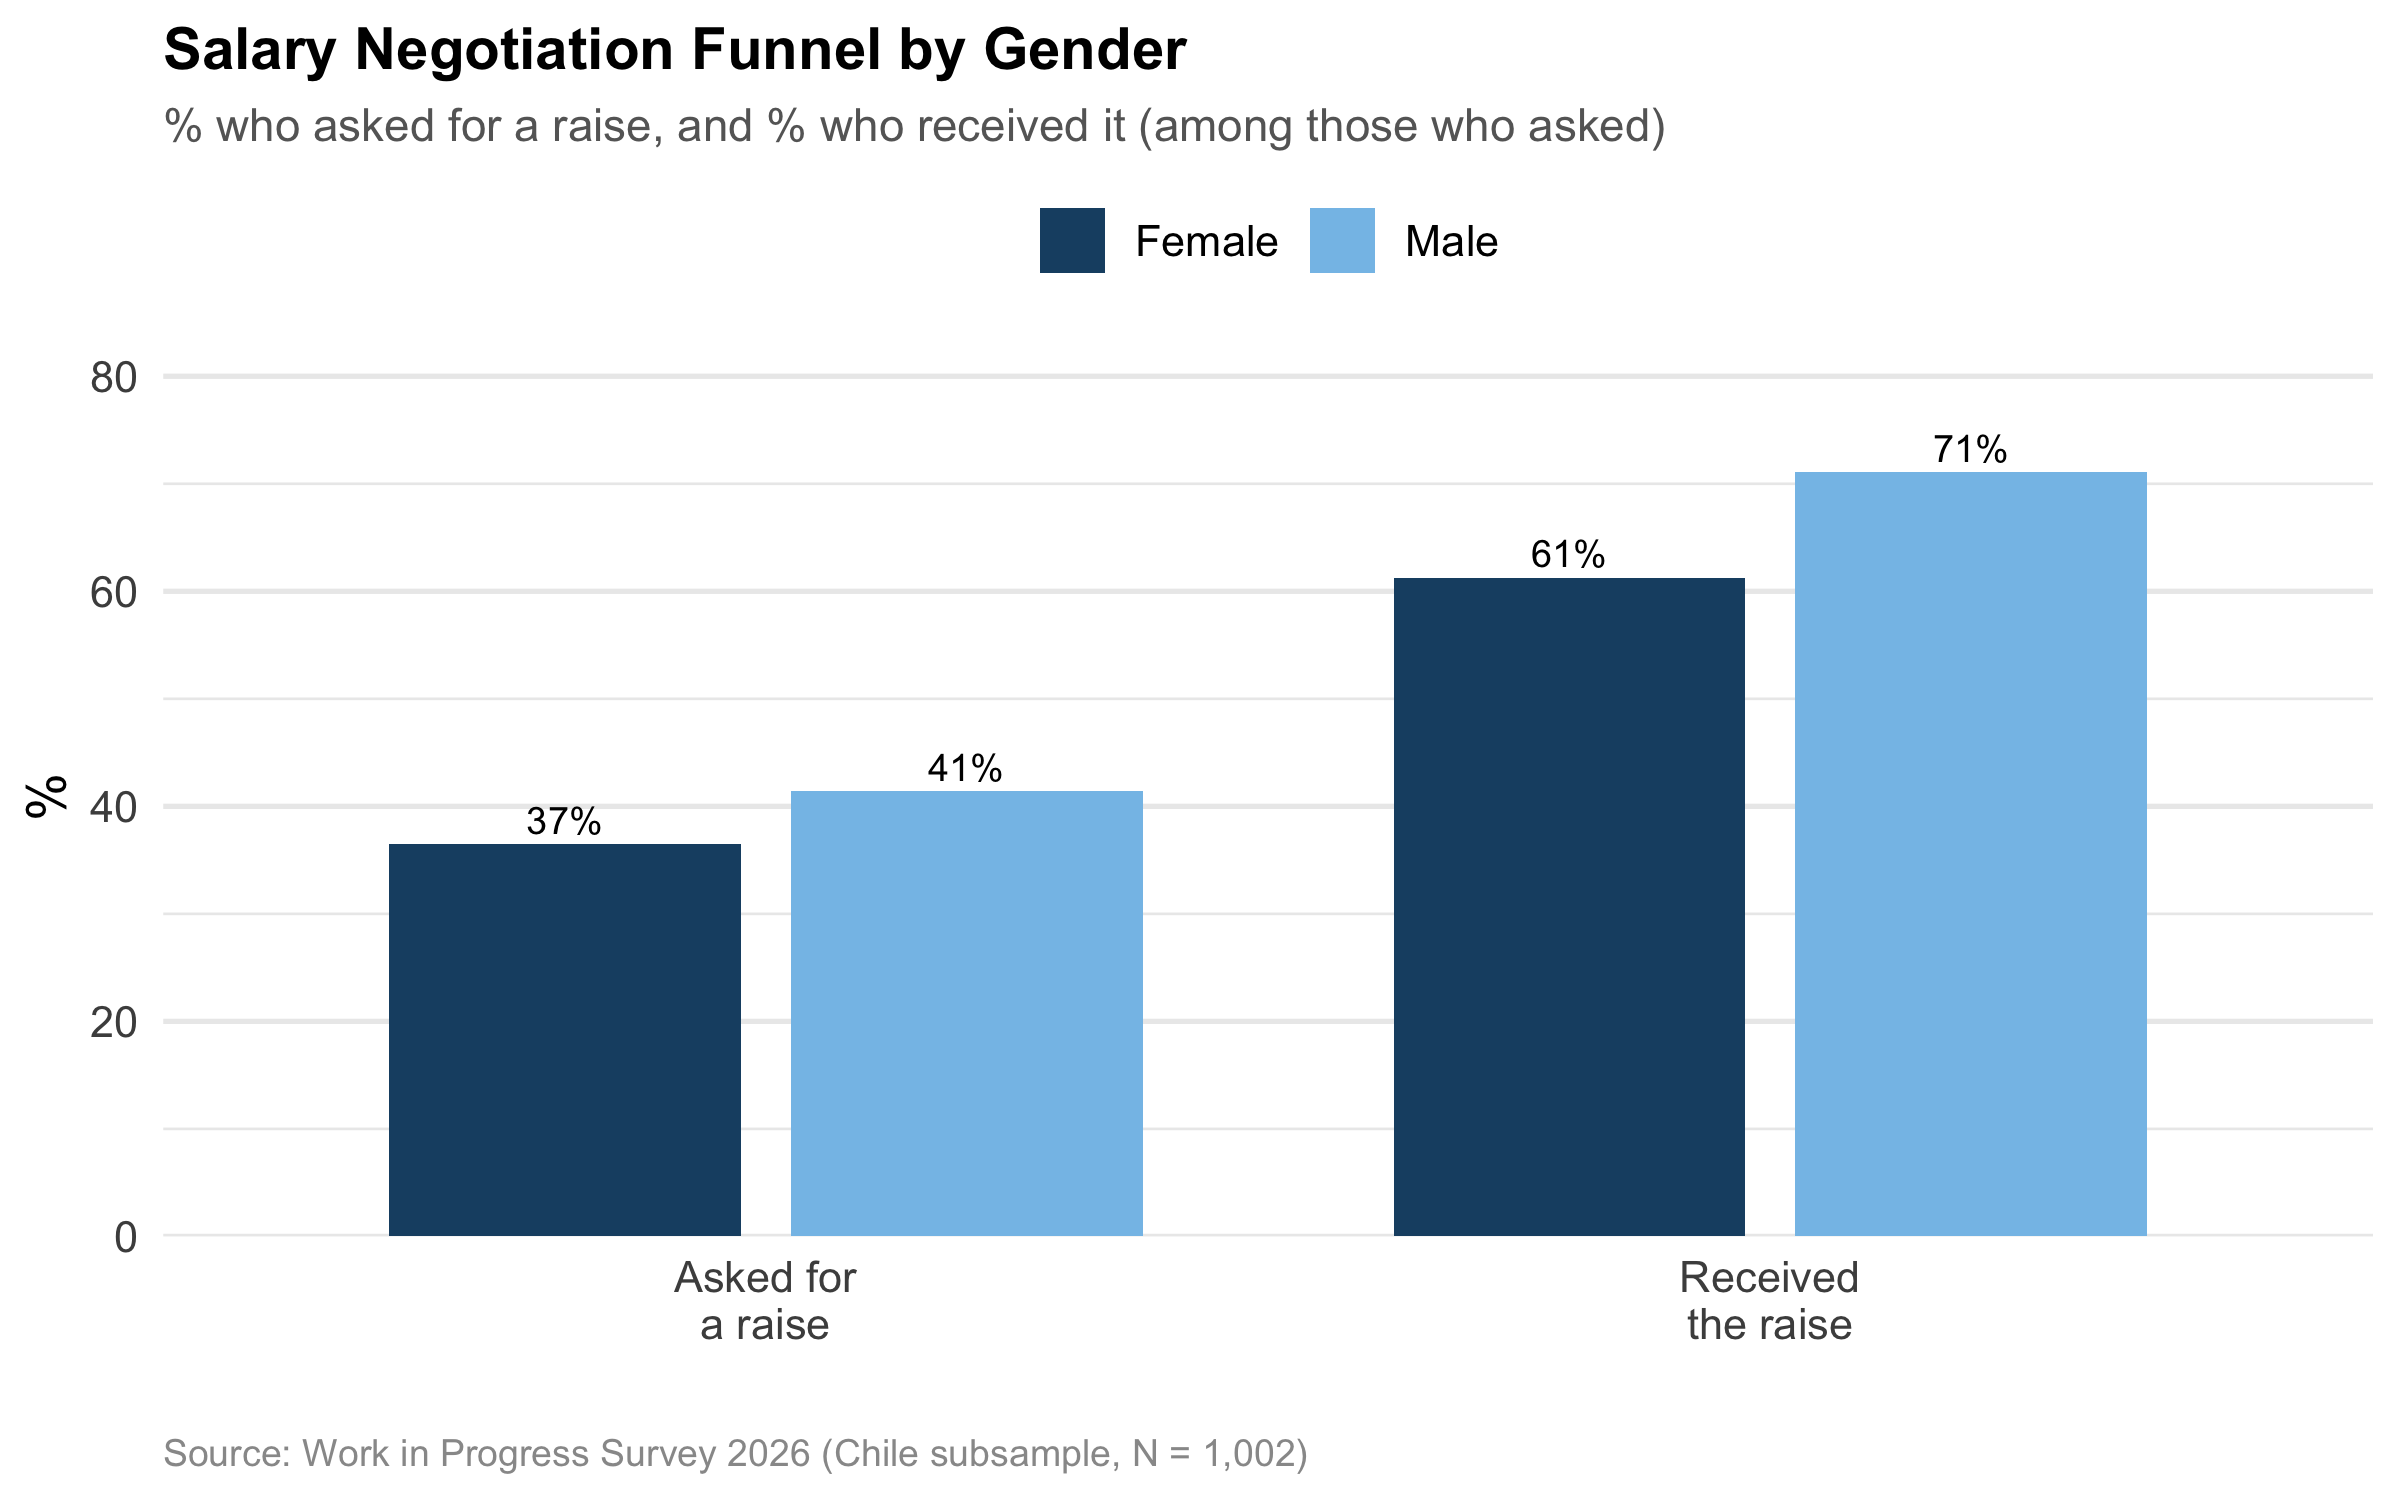
\includegraphics[width=0.65\textwidth]{rf_5_2_negotiation_funnel_by_gender.png}
\end{center}

\vspace{-0.1cm}
\small
Women are less likely to ask for a raise, and conditional on asking, less likely to receive one. Source: WiP Survey 2026, Chile subsample (N = 1,002).

\end{frame}

\begin{frame}
\frametitle{Perceived promotion opportunities by gender}

\begin{center}
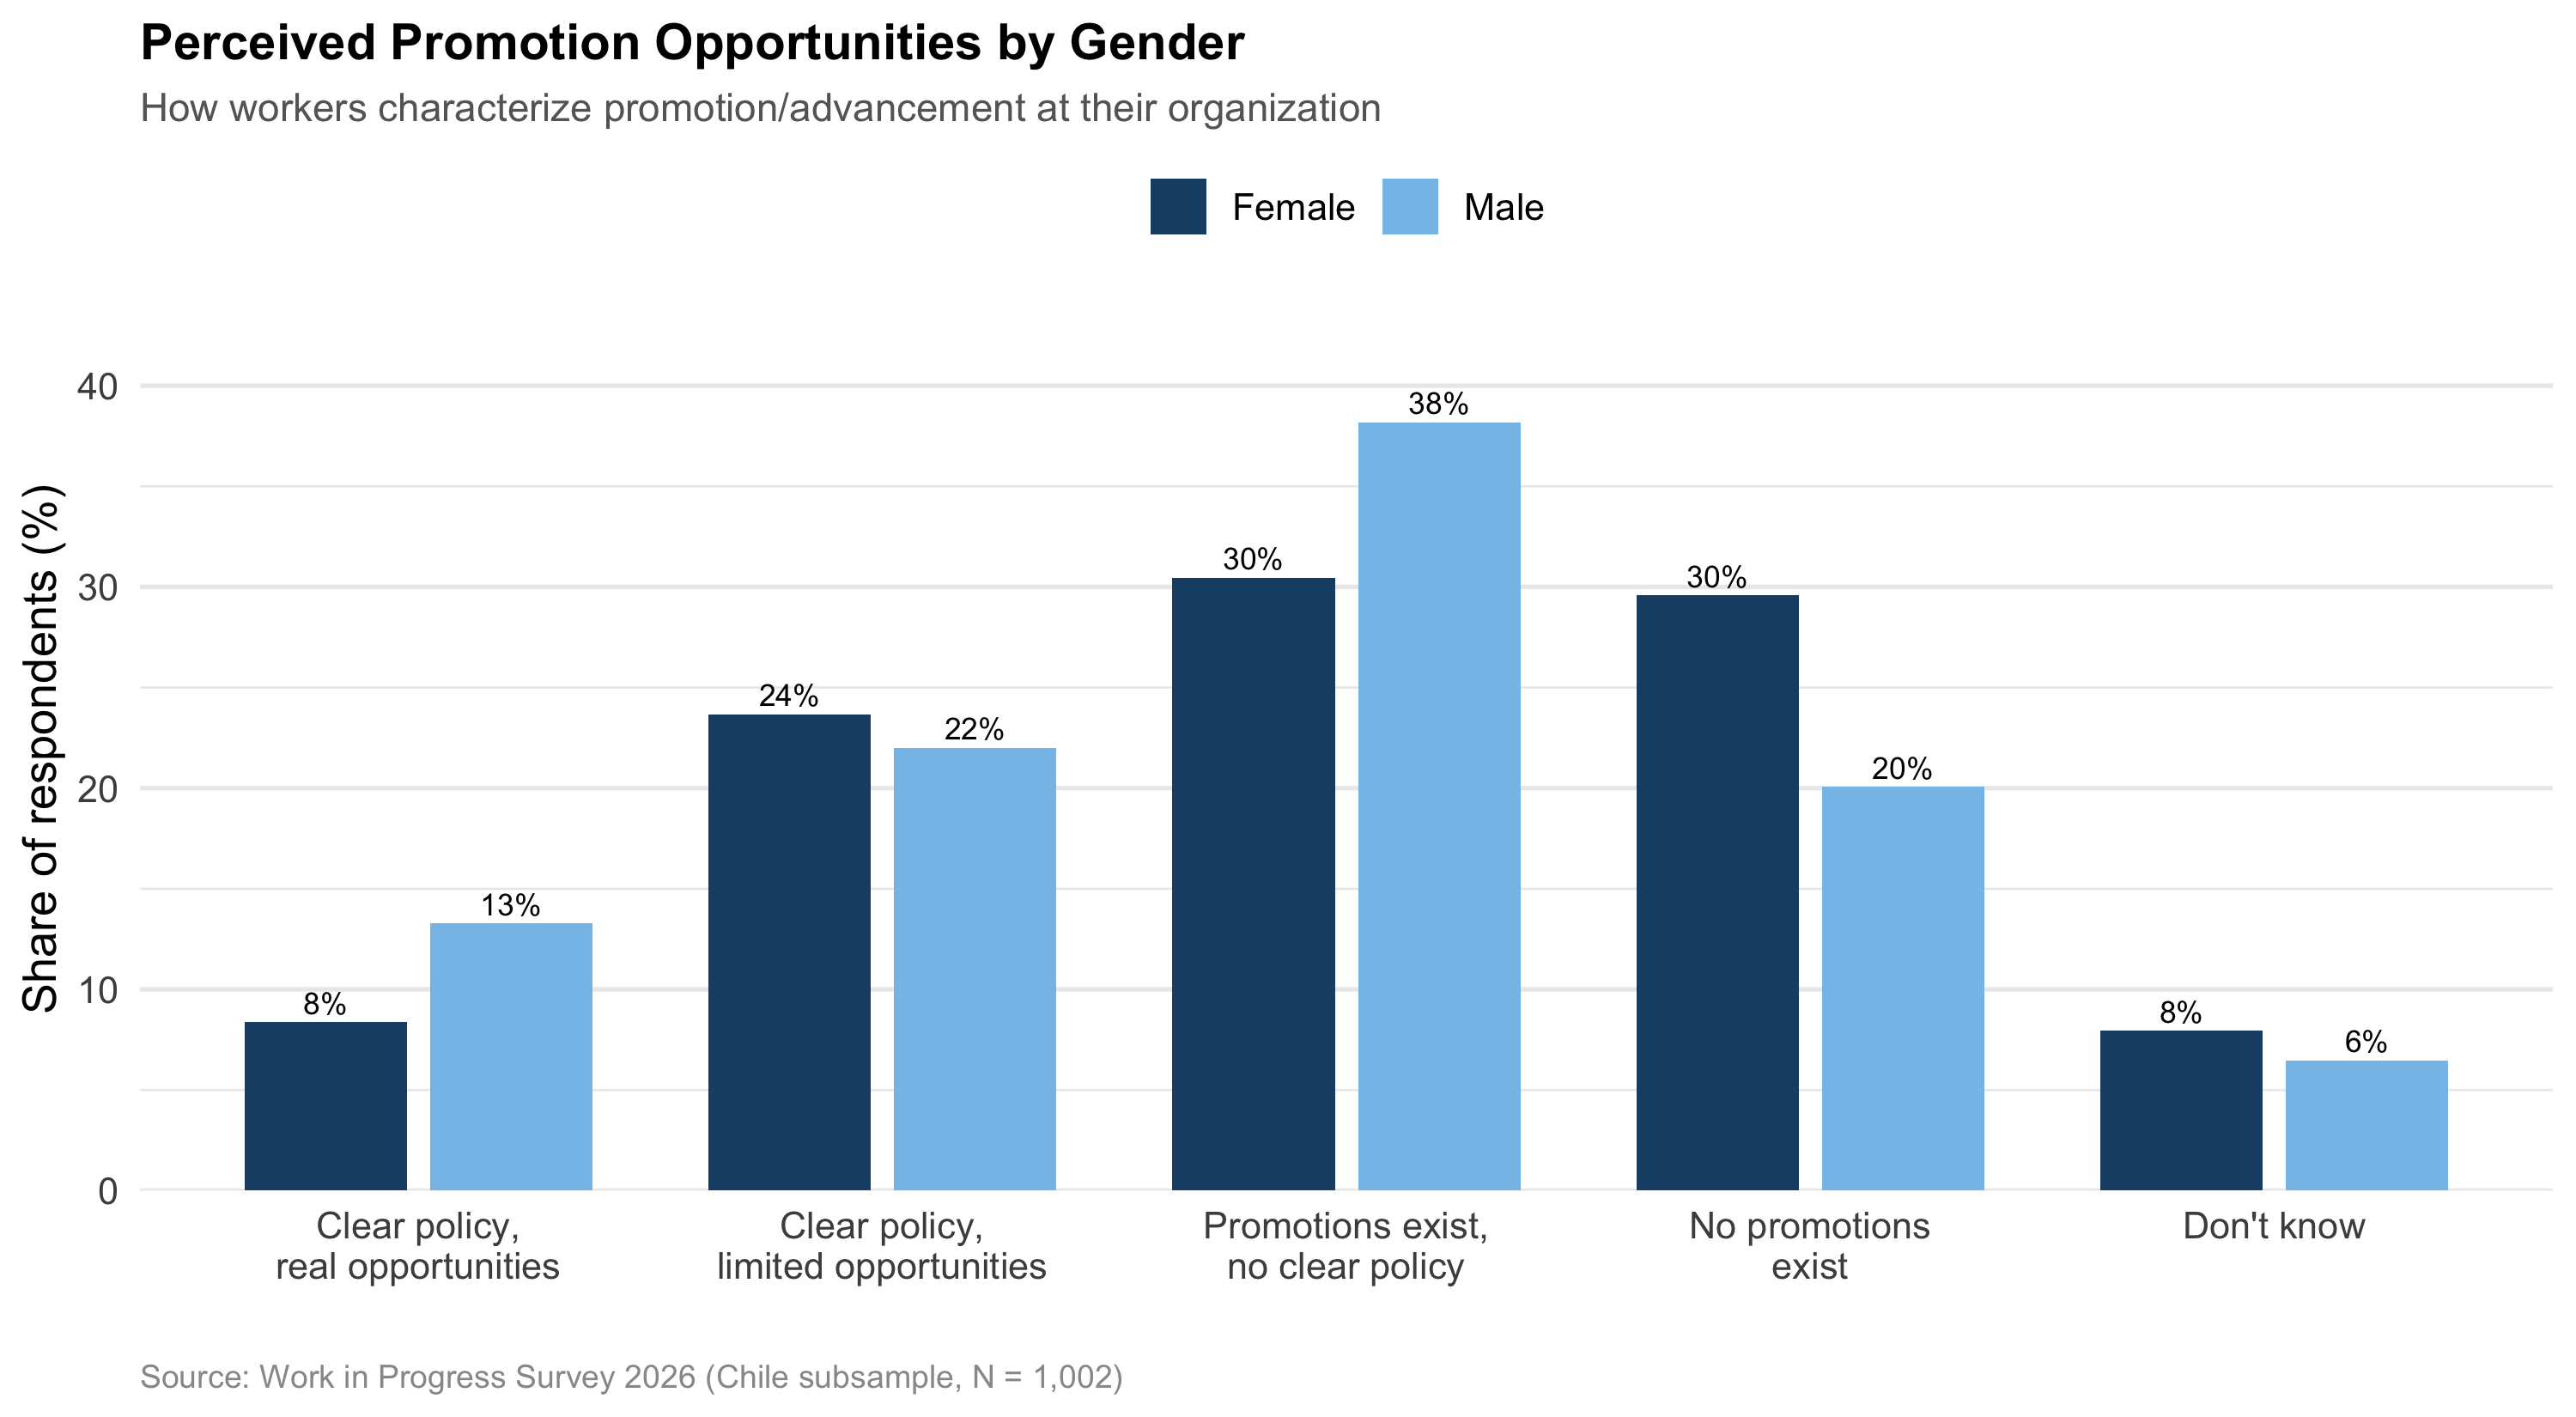
\includegraphics[width=0.65\textwidth]{rf_1_7_promotion_perceptions_by_gender.png}
\end{center}

\vspace{-0.1cm}
\small
Women report fewer promotion opportunities at their organization. Source: WiP Survey 2026, Chile subsample (N = 1,002).

\end{frame}

\begin{frame}
\frametitle{Promotion negotiation funnel by gender (2025)}

\begin{center}
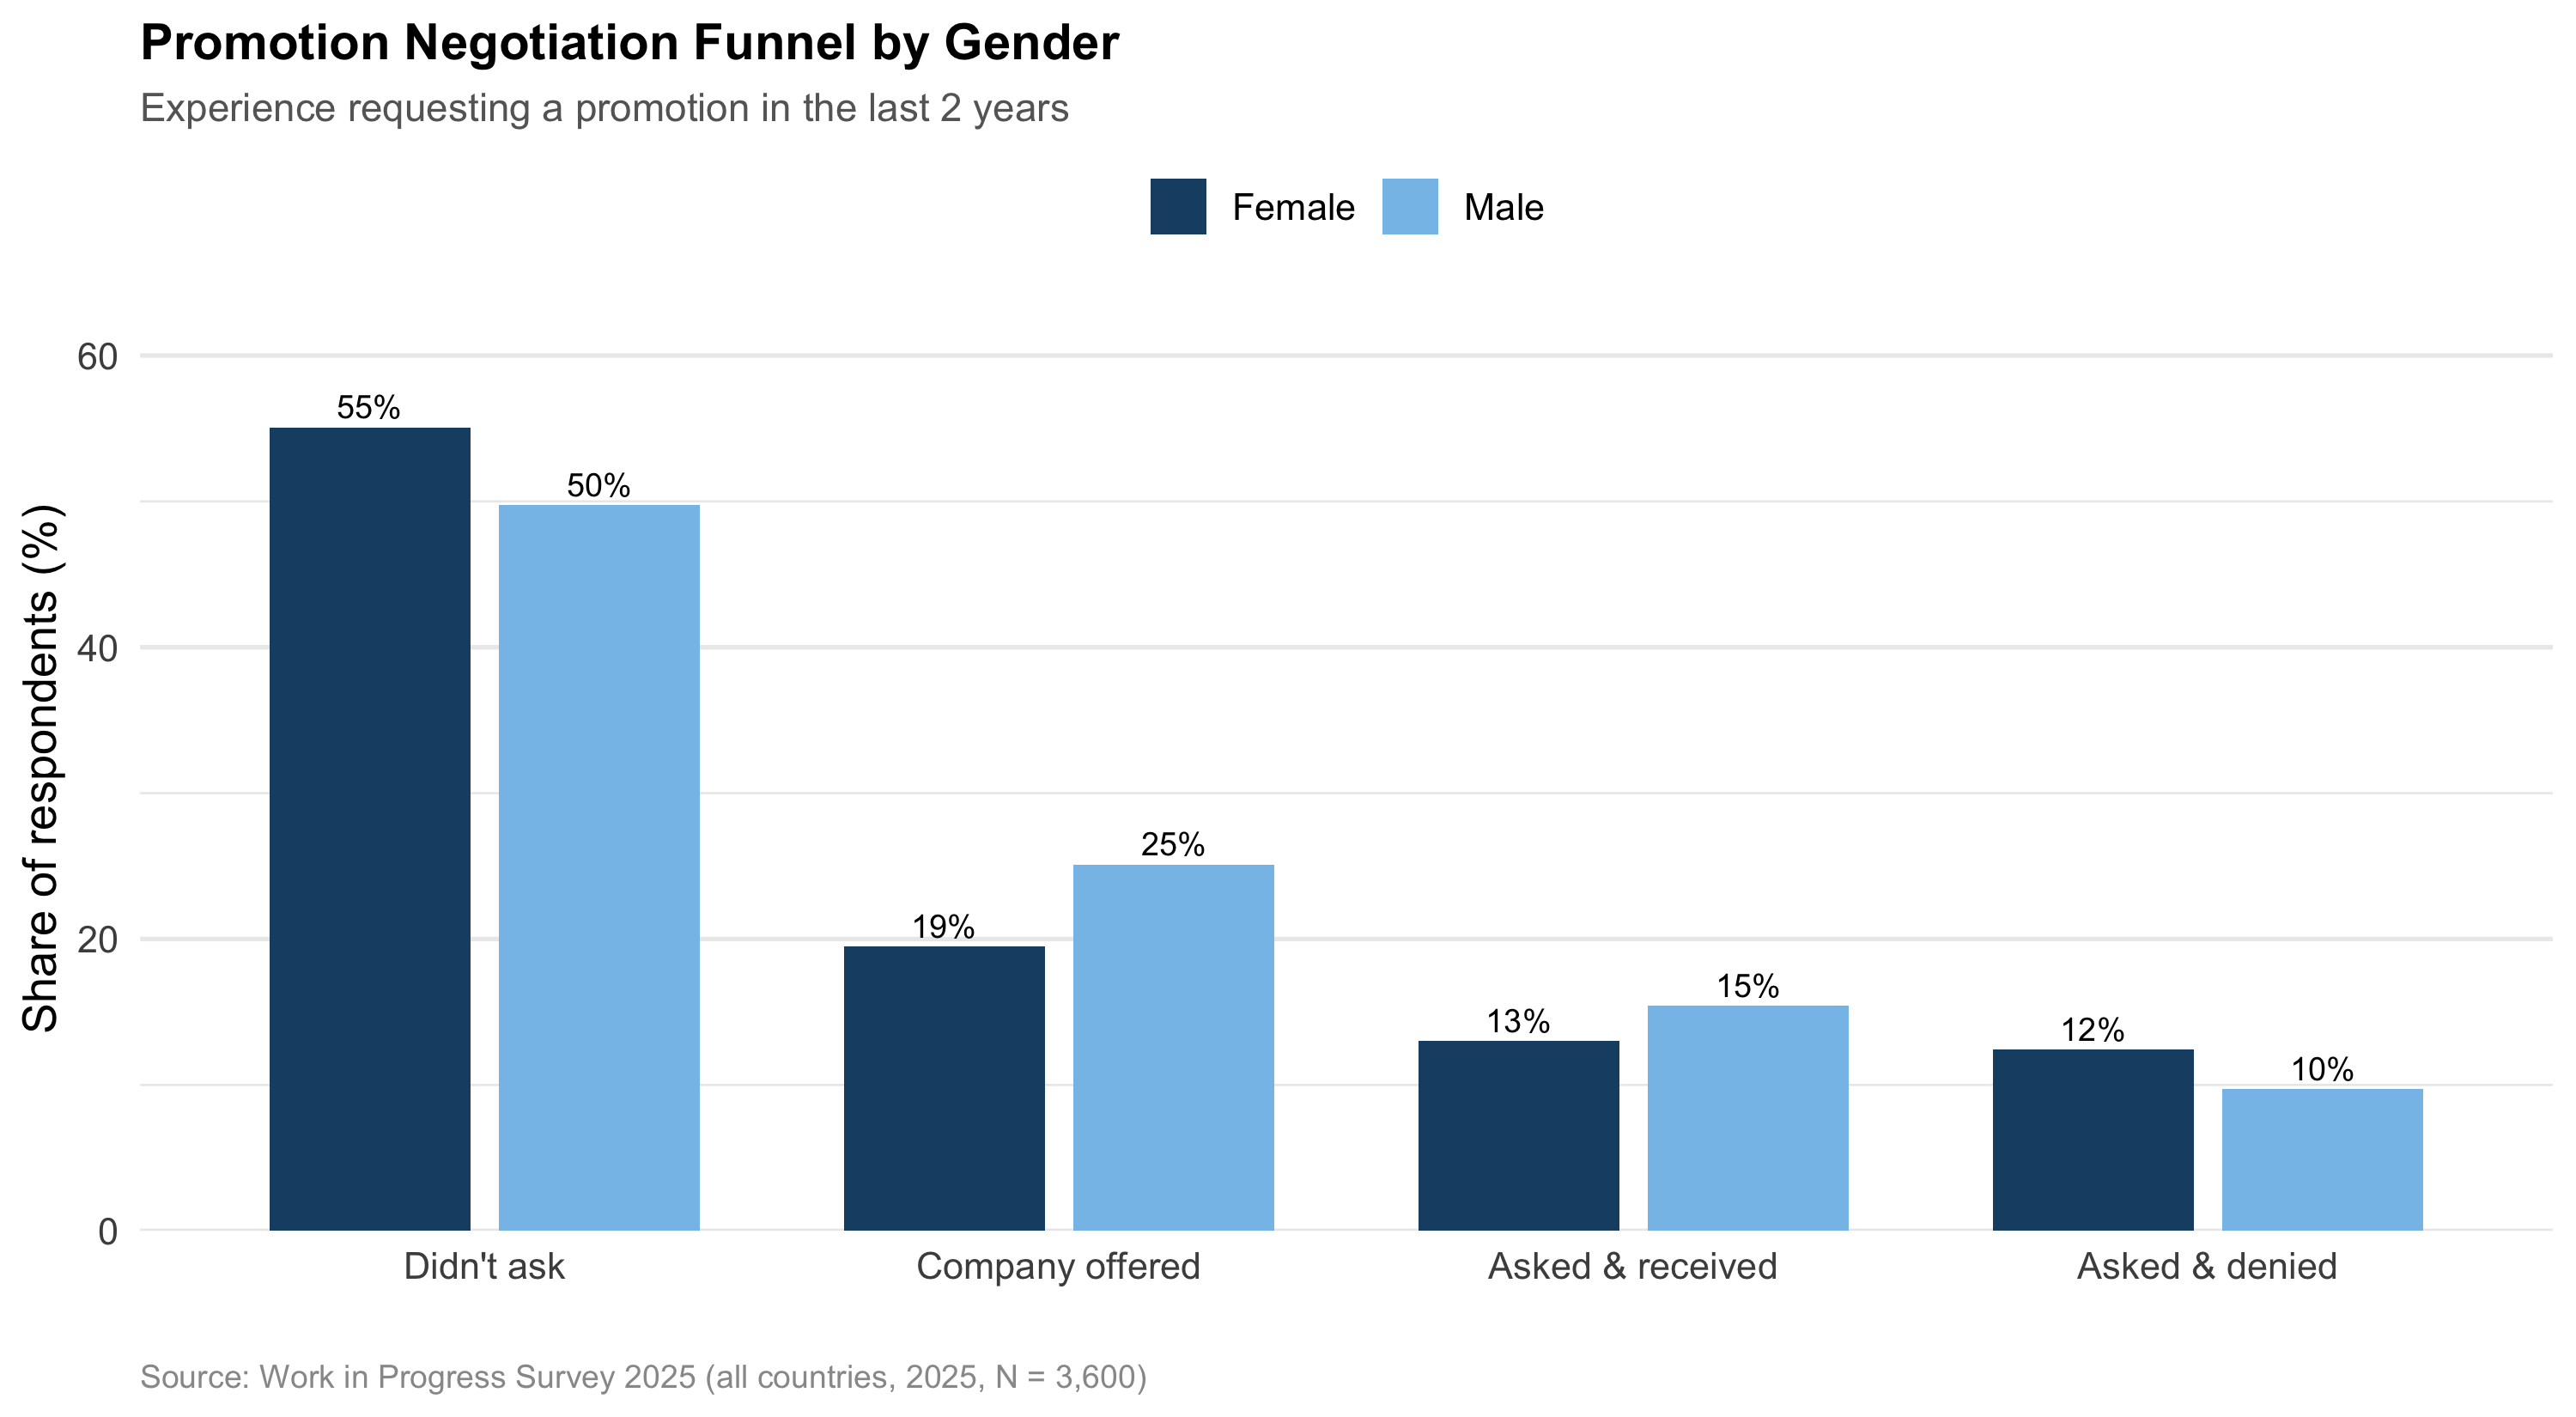
\includegraphics[width=0.65\textwidth]{rf25_all_5_7_promotion_funnel_by_gender.png}
\end{center}

\vspace{-0.1cm}
\small
Women are more likely to ask for a promotion but more likely to be denied (12\% F vs.\ 10\% M). Men receive unsolicited promotions more often (25\% vs.\ 19\%). Source: WiP Survey 2025, all countries (N = 3,600).

\end{frame}

\begin{frame}
\frametitle{Salary negotiation funnel by gender (2025)}

\begin{center}
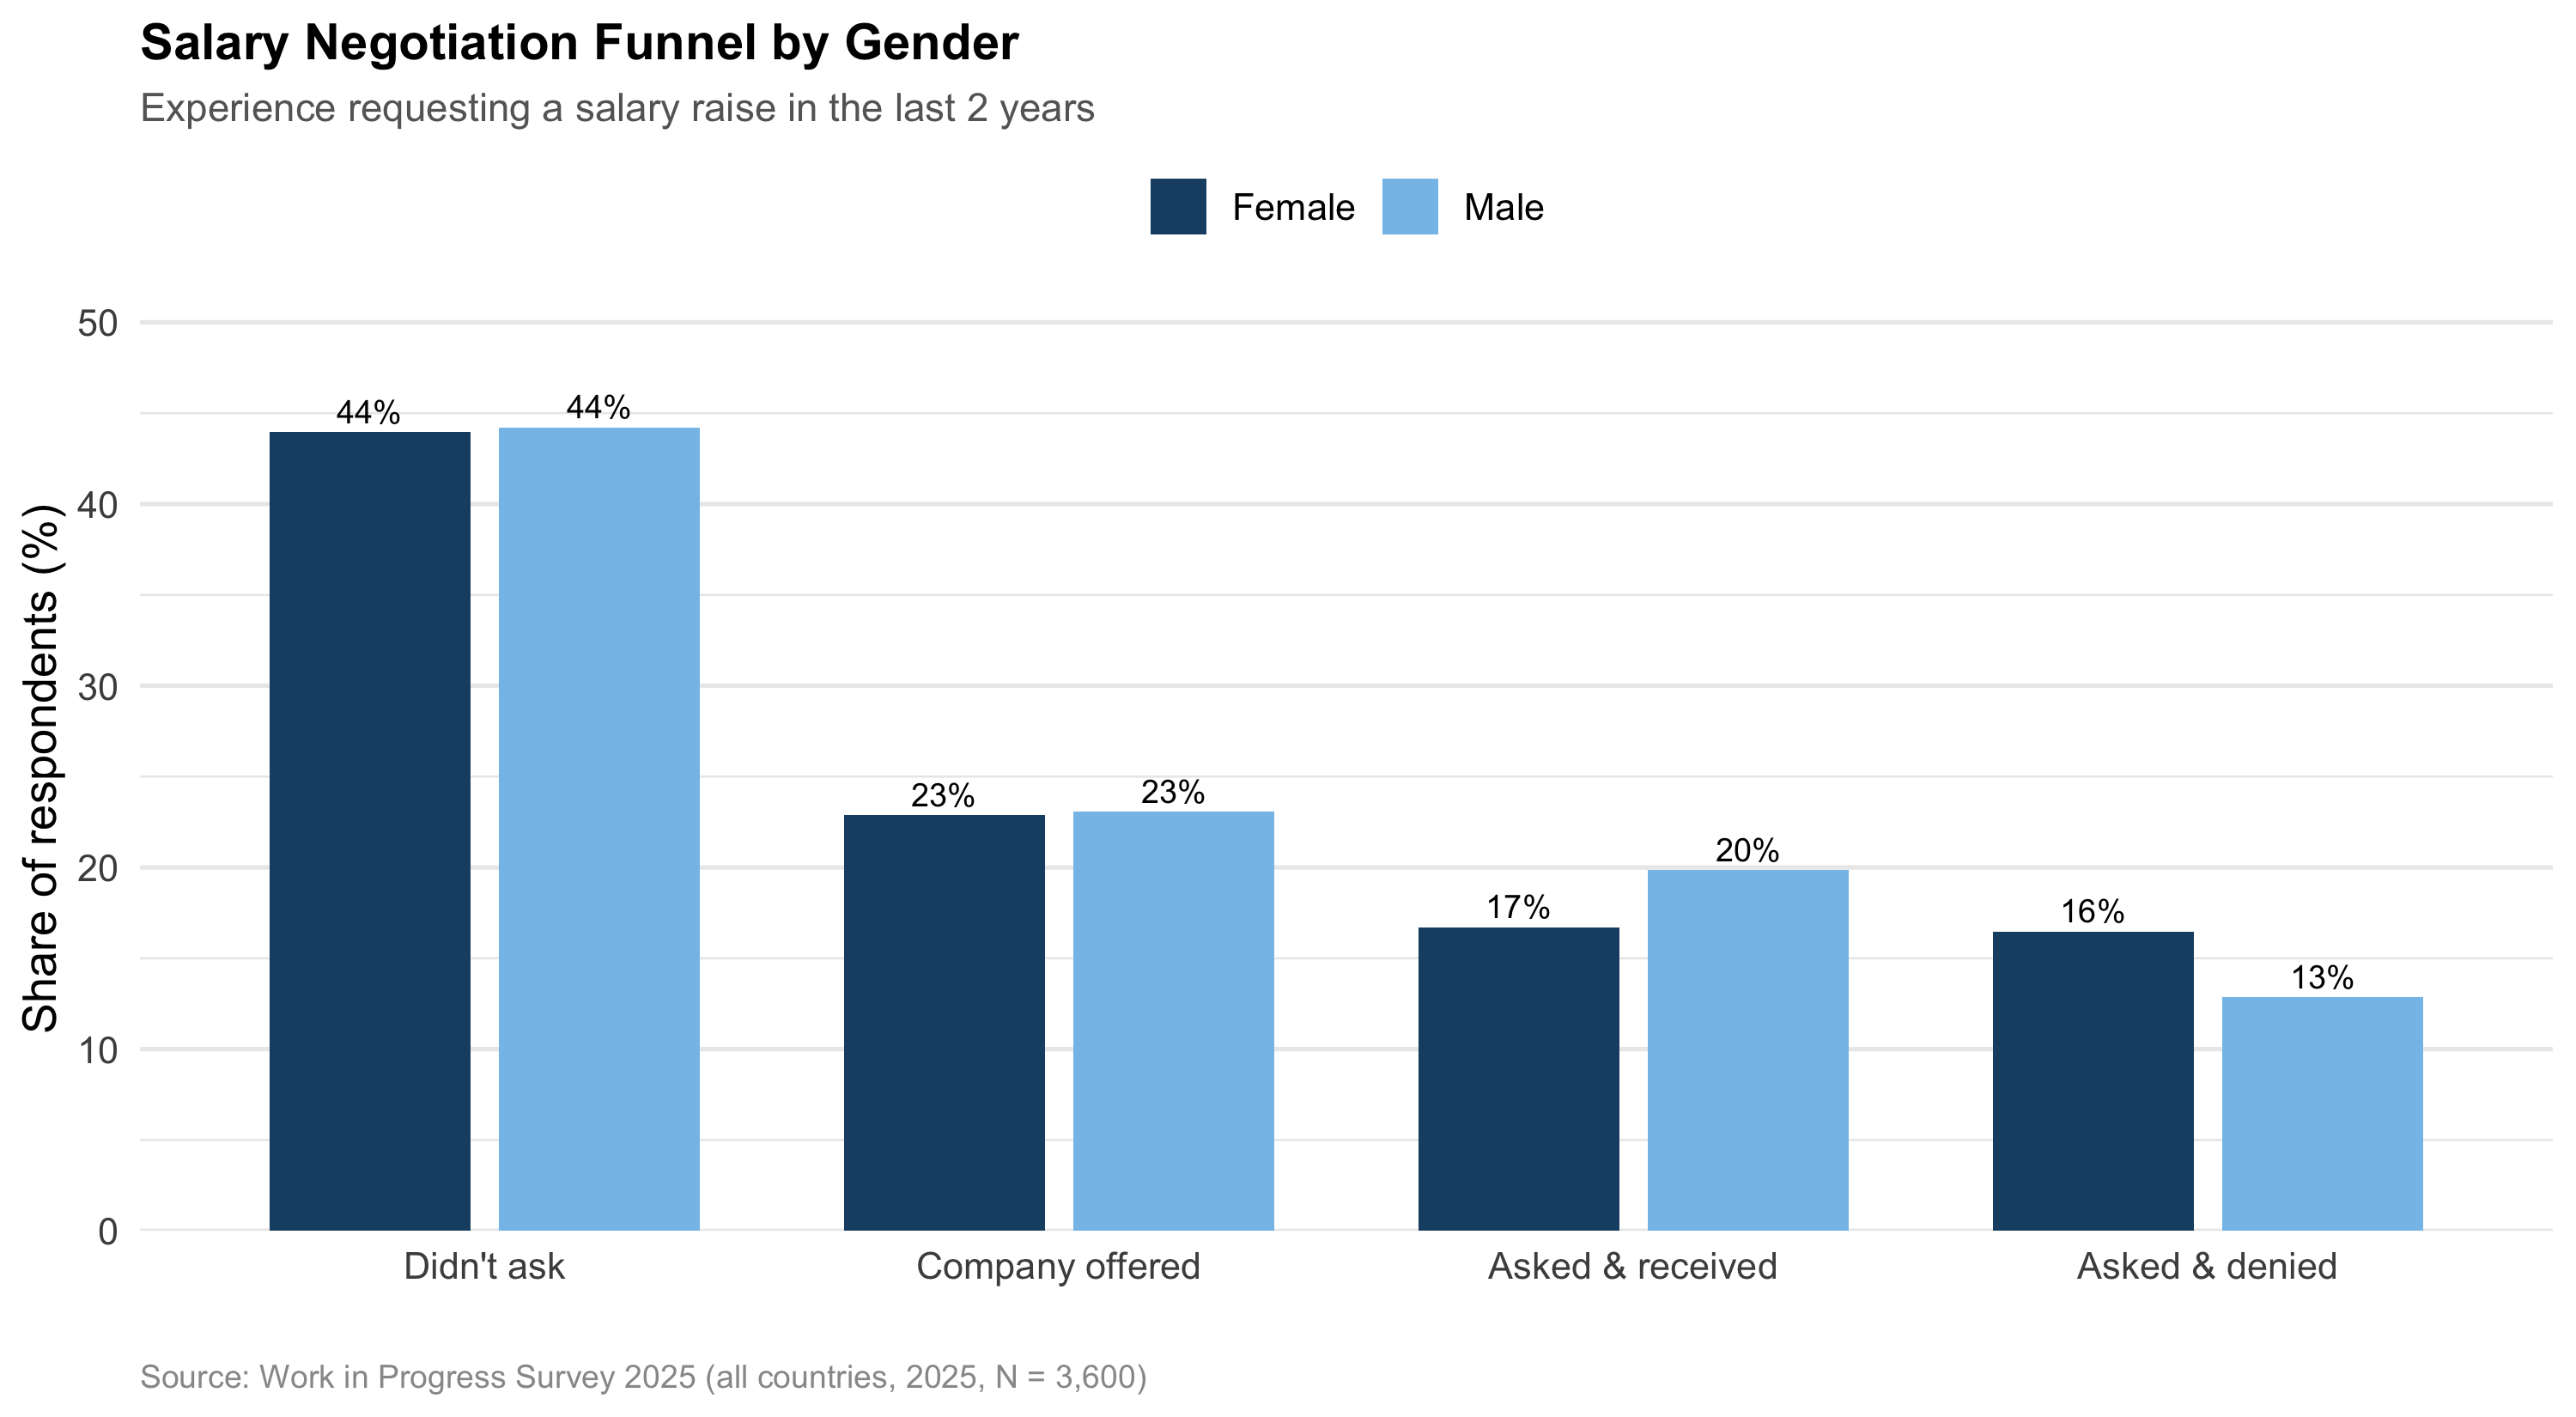
\includegraphics[width=0.65\textwidth]{rf25_all_5_9_salary_funnel_by_gender.png}
\end{center}

\vspace{-0.1cm}
\small
Equal shares didn't ask (44\%) and received unsolicited raises (23\%), but women who asked were less likely to receive (17\% F vs.\ 20\% M) and more likely to be denied (16\% F vs.\ 13\% M). Source: WiP Survey 2025, all countries (N = 3,600).

\end{frame}

\end{document}
